


\section{Caracterizaci\'on de componentes pasivos}
En esta secci\'on se analiza el comportamiento de los componentes pasivos en funci\'on de la frecuencia de operaci\'on, en particular de un capacitor y un inductor.
Para dicho an\'alisis se realiza un barrido en frecuencias desde $10Hz$ a $10MHz$.

\subsection{Medici\'on del capacitor}
Para la medici\'on se utiliza un capacitor de $22nF$ de film y se configura el analizador de impedancias en modelo paralelo para medir fase y admitancia. En este caso, debido a las caracter\'isticas particulares del componente, no es posible realizar el barrido de frecuencias completo.
\subsubsection{Resultados}
Se muestran en la Tabla \ref{tab:Med_CAP}  los resultados obtenidos de las mediciones y en la Figura \ref{fig:Med_CAP} los respectivos  gr\'aficos realizados a partir de estas.

\begin{table}[H]
    \centering
    \resizebox{0.5\textwidth}{!}{%
        \begin{tabular}{ccccc}
            \hline
            \begin{tabular}[c]{@{}c@{}}Frecuencia\\   (Hz)\end{tabular} & Capacidad (F) & \begin{tabular}[c]{@{}c@{}}Factor de\\   disipación\end{tabular} & Admitancia (s) & Fase ($^\circ$) \\ \hline
            5 & 2.20E-08 & 0.006 & 6.80E-07 & 89.5 \\
            10 & 2.19E-08 & 0.006 & 1.38E-06 & 89.9 \\
            20 & 2.20E-08 & 0 & 2.76E-06 & 90 \\
            100 & 2.19E-08 & 0.0012 & 1.38E-05 & 89.93 \\
            300 & 2.19E-08 & 0.0025 & 4.13E-05 & 89.86 \\
            1000 & 2.19E-08 & 0.0039 & 1.37E-04 & 89.78 \\
            3000 & 2.18E-08 & 0.0064 & 4.10E-04 & 89.64 \\
            10000 & 2.17E-08 & 0.0086 & 1.36E-03 & 89.51 \\
            30000 & 2.15E-08 & 0.0124 & 4.05E-03 & 89.29 \\
            80000 & 2.13E-08 & 0.0157 & 1.07E-02 & 89.1 \\
            100000 & 2.13E-08 & 0.0165 & 1.34E-02 & 89.06 \\
            150000 & 2.12E-08 & 0.018 & 2.00E-02 & 88.97 \\
            200000 & 2.11E-08 & 0.0191 & 2.66E-02 & 88.91 \\
            300000 & 2.11E-08 & 0.0211 & 3.97E-02 & 88.79 \\
            400000 & 2.10E-08 & 0.0228 & 5.28E-02 & 88.69 \\
            500000 & 2.10E-08 & 0.0245 & 6.60E-02 & 88.6 \\
            600000 & 2.10E-08 & 0.0262 & 7.91E-02 & 88.5 \\
            700000 & 2.10E-08 & 0.0279 & 9.24E-02 & 88.4 \\
            750000 & 2.10E-08 & 0.0287 & 9.90E-02 & 88.35 \\
            780000 & 2.10E-08 & 0.0292 & 1.03E-01 & 88.32 \\
            800000 & 2.10E-08 & 0.0296 & 1.06E-01 & 88.31 \\
            825000 & 2.10E-08 & 0.03 & 1.09E-01 & 88.28 \\
            850000 & 2.10E-08 & 0.0305 & 1.12E-01 & 88.25 \\
            900000 & 2.11E-08 & 0.0313 & 1.19E-01 & 88.18 \\
            1000000 & 2.11E-08 & 0.033 & 0.133 & 88.1 \\
            2000000 & 2.19E-08 & 0.052 & 0.276 & 87 \\
            3000000 & 2.36E-08 & 0.077 & 0.447 & 85.6 \\
            4000000 & 2.66E-08 & 0.112 & 0.673 & 83.6 \\
            5000000 & 3.18E-08 & 0.166 & 1.012 & 80.6 \\
             \hline
        \end{tabular}%
    }
    \caption{Mediciones del capacitor}
    \label{tab:Med_CAP}
\end{table}

\begin{figure}[H]
    \centering
    \resizebox{\textwidth}{!}{
        \begin{tabular}{c c}
            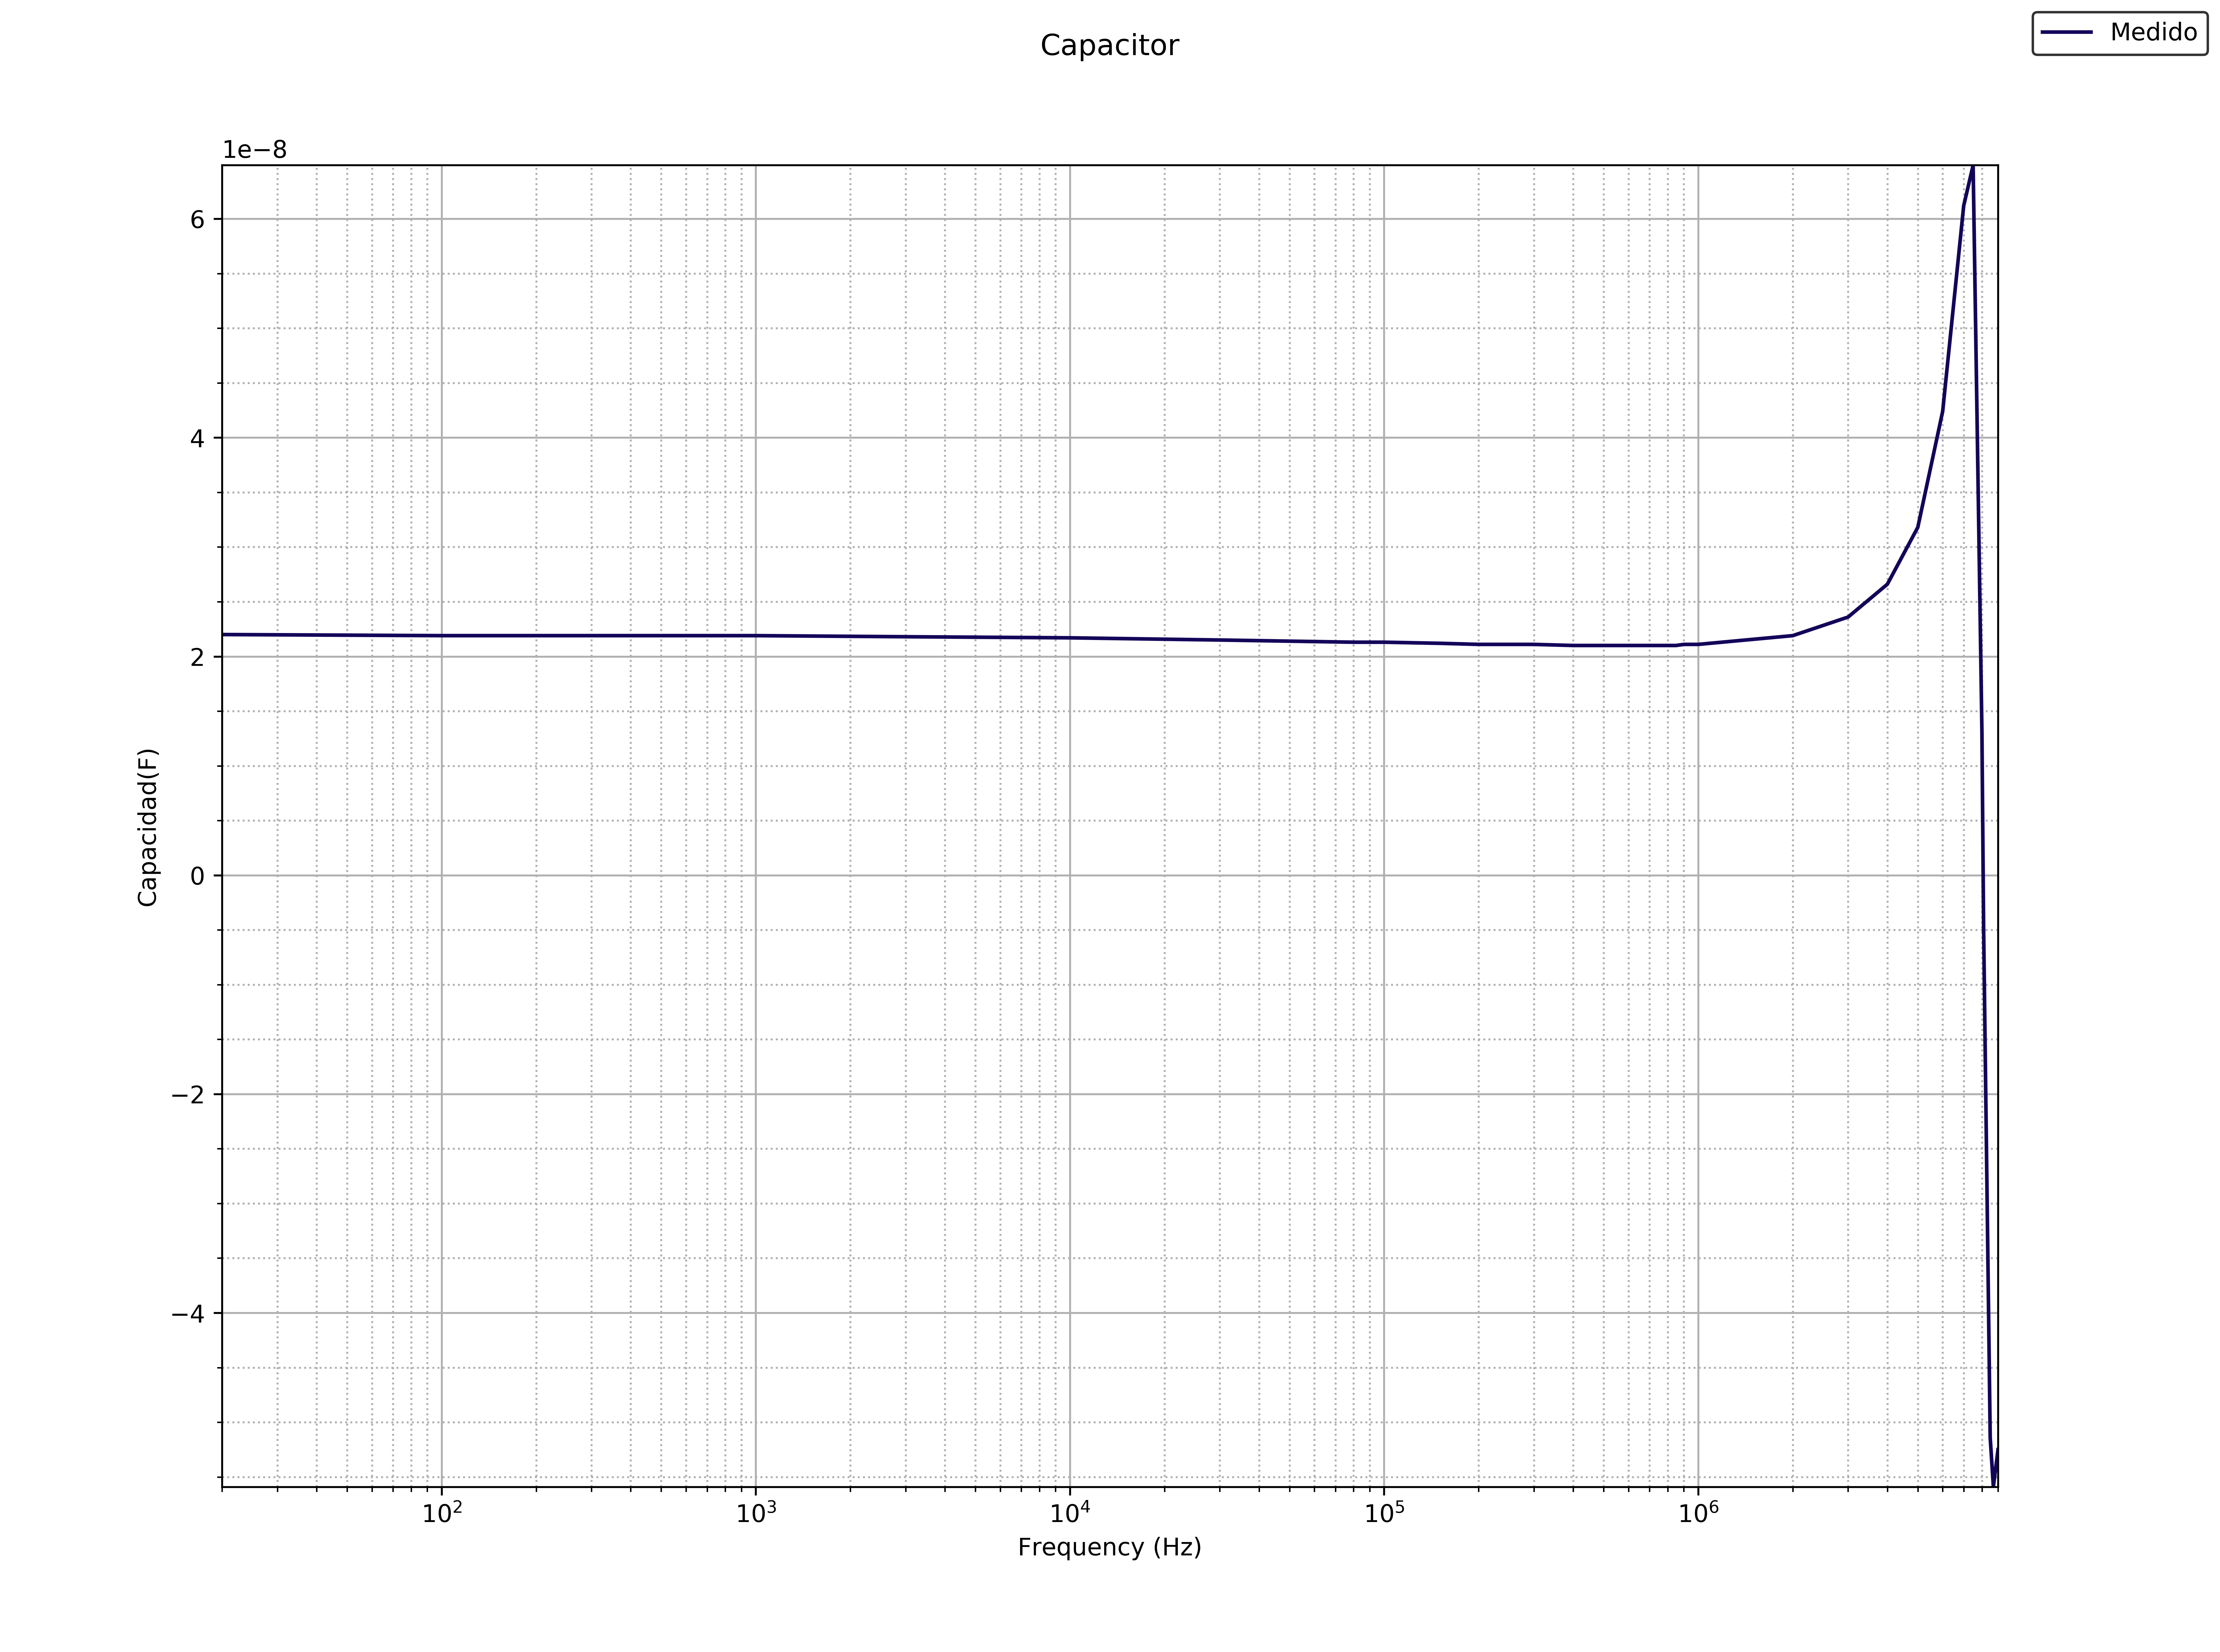
\includegraphics{Recursos/capacidad_medida.png}&
            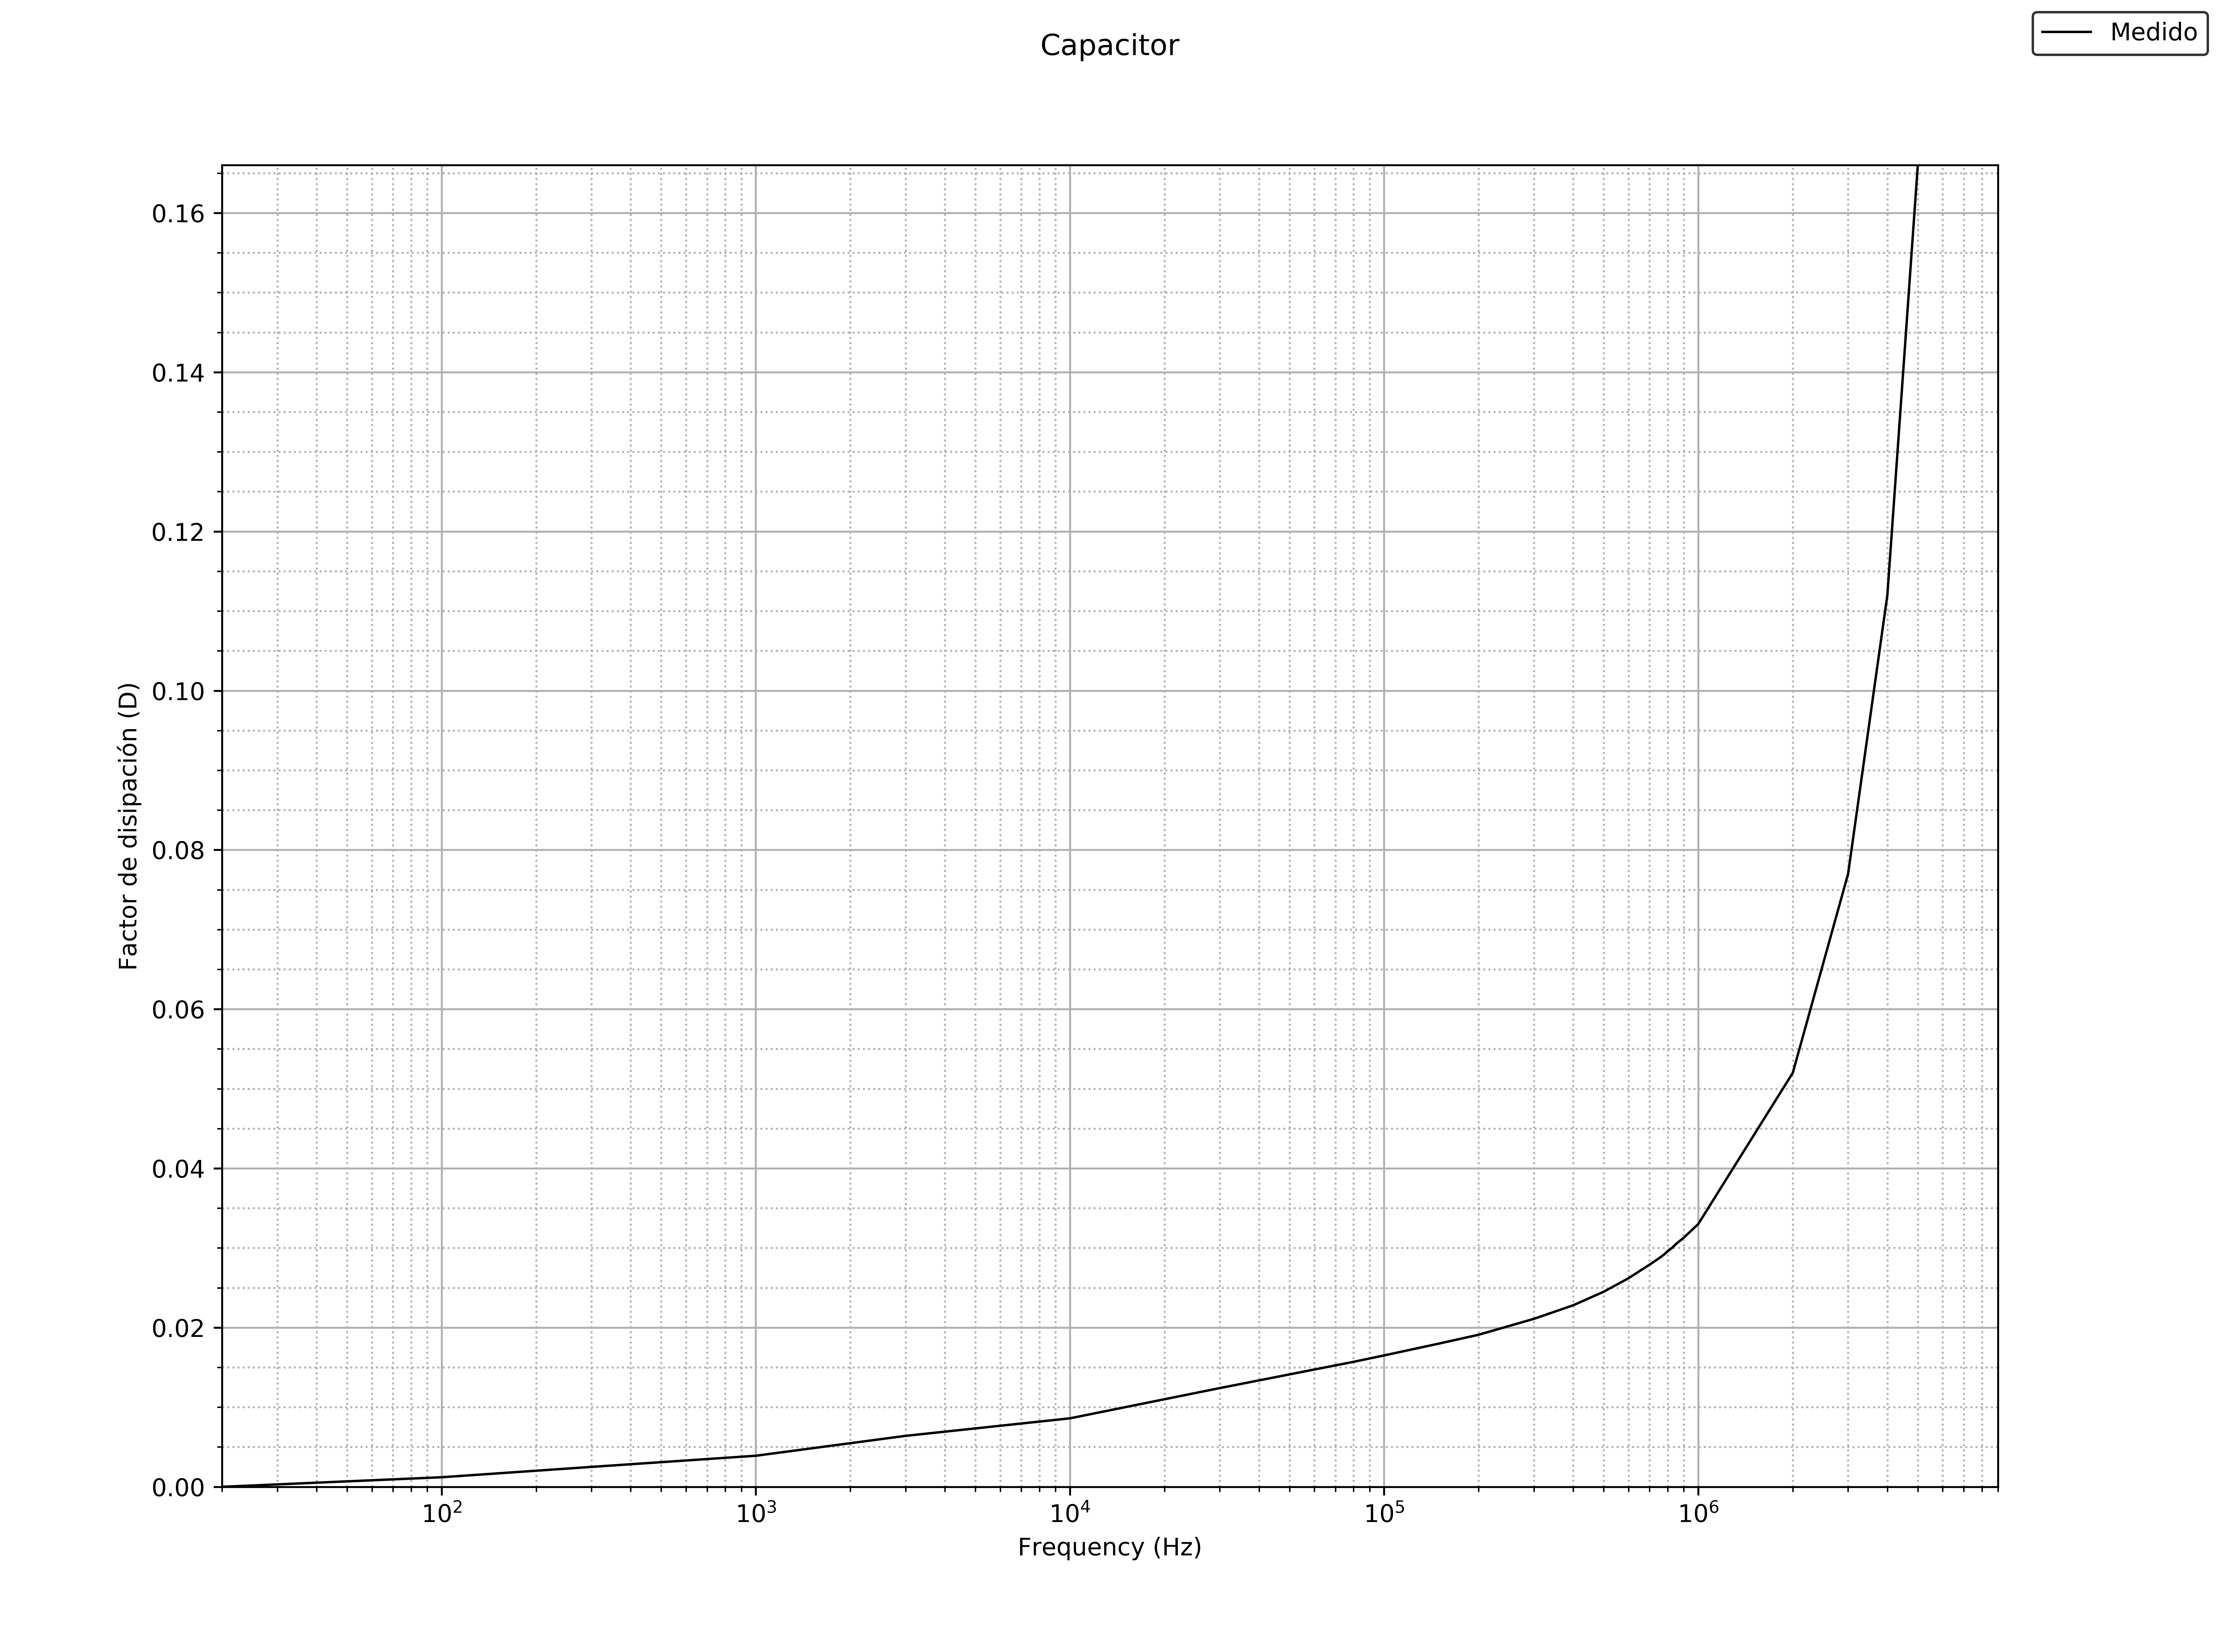
\includegraphics{Recursos/perdidas_medida_cap.png} \\
            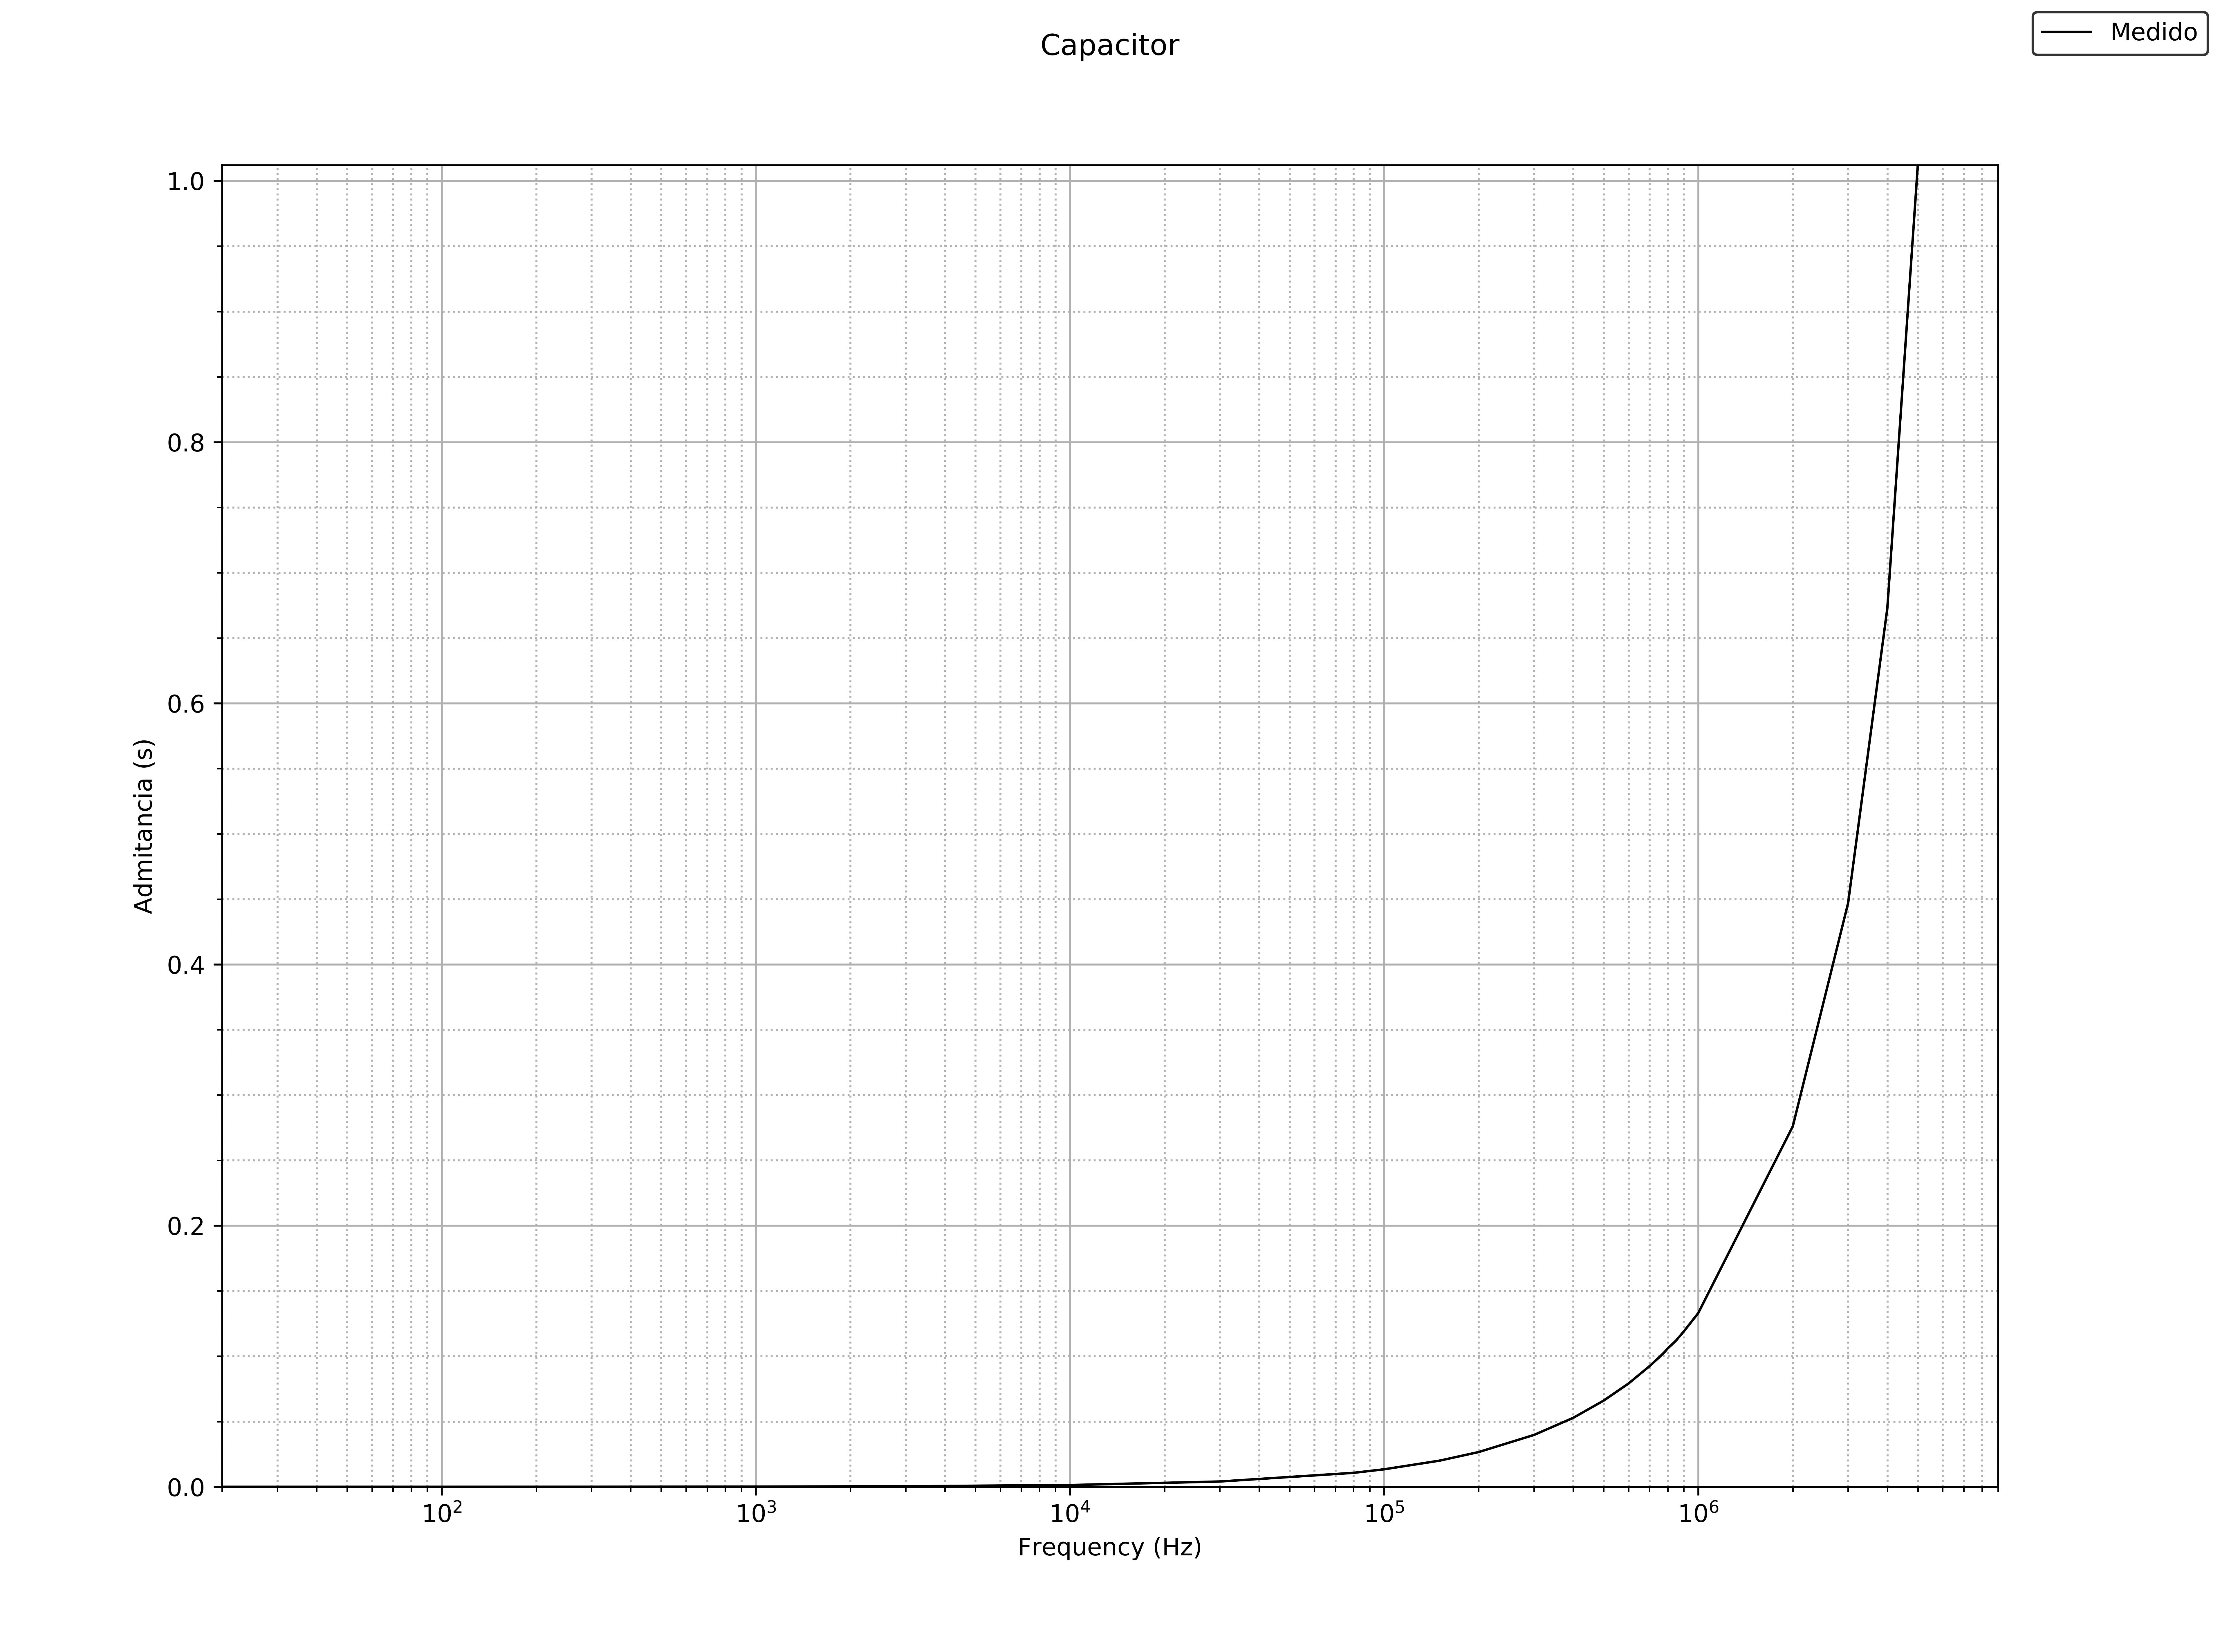
\includegraphics{Recursos/admitancia_medida_cap.png} &
            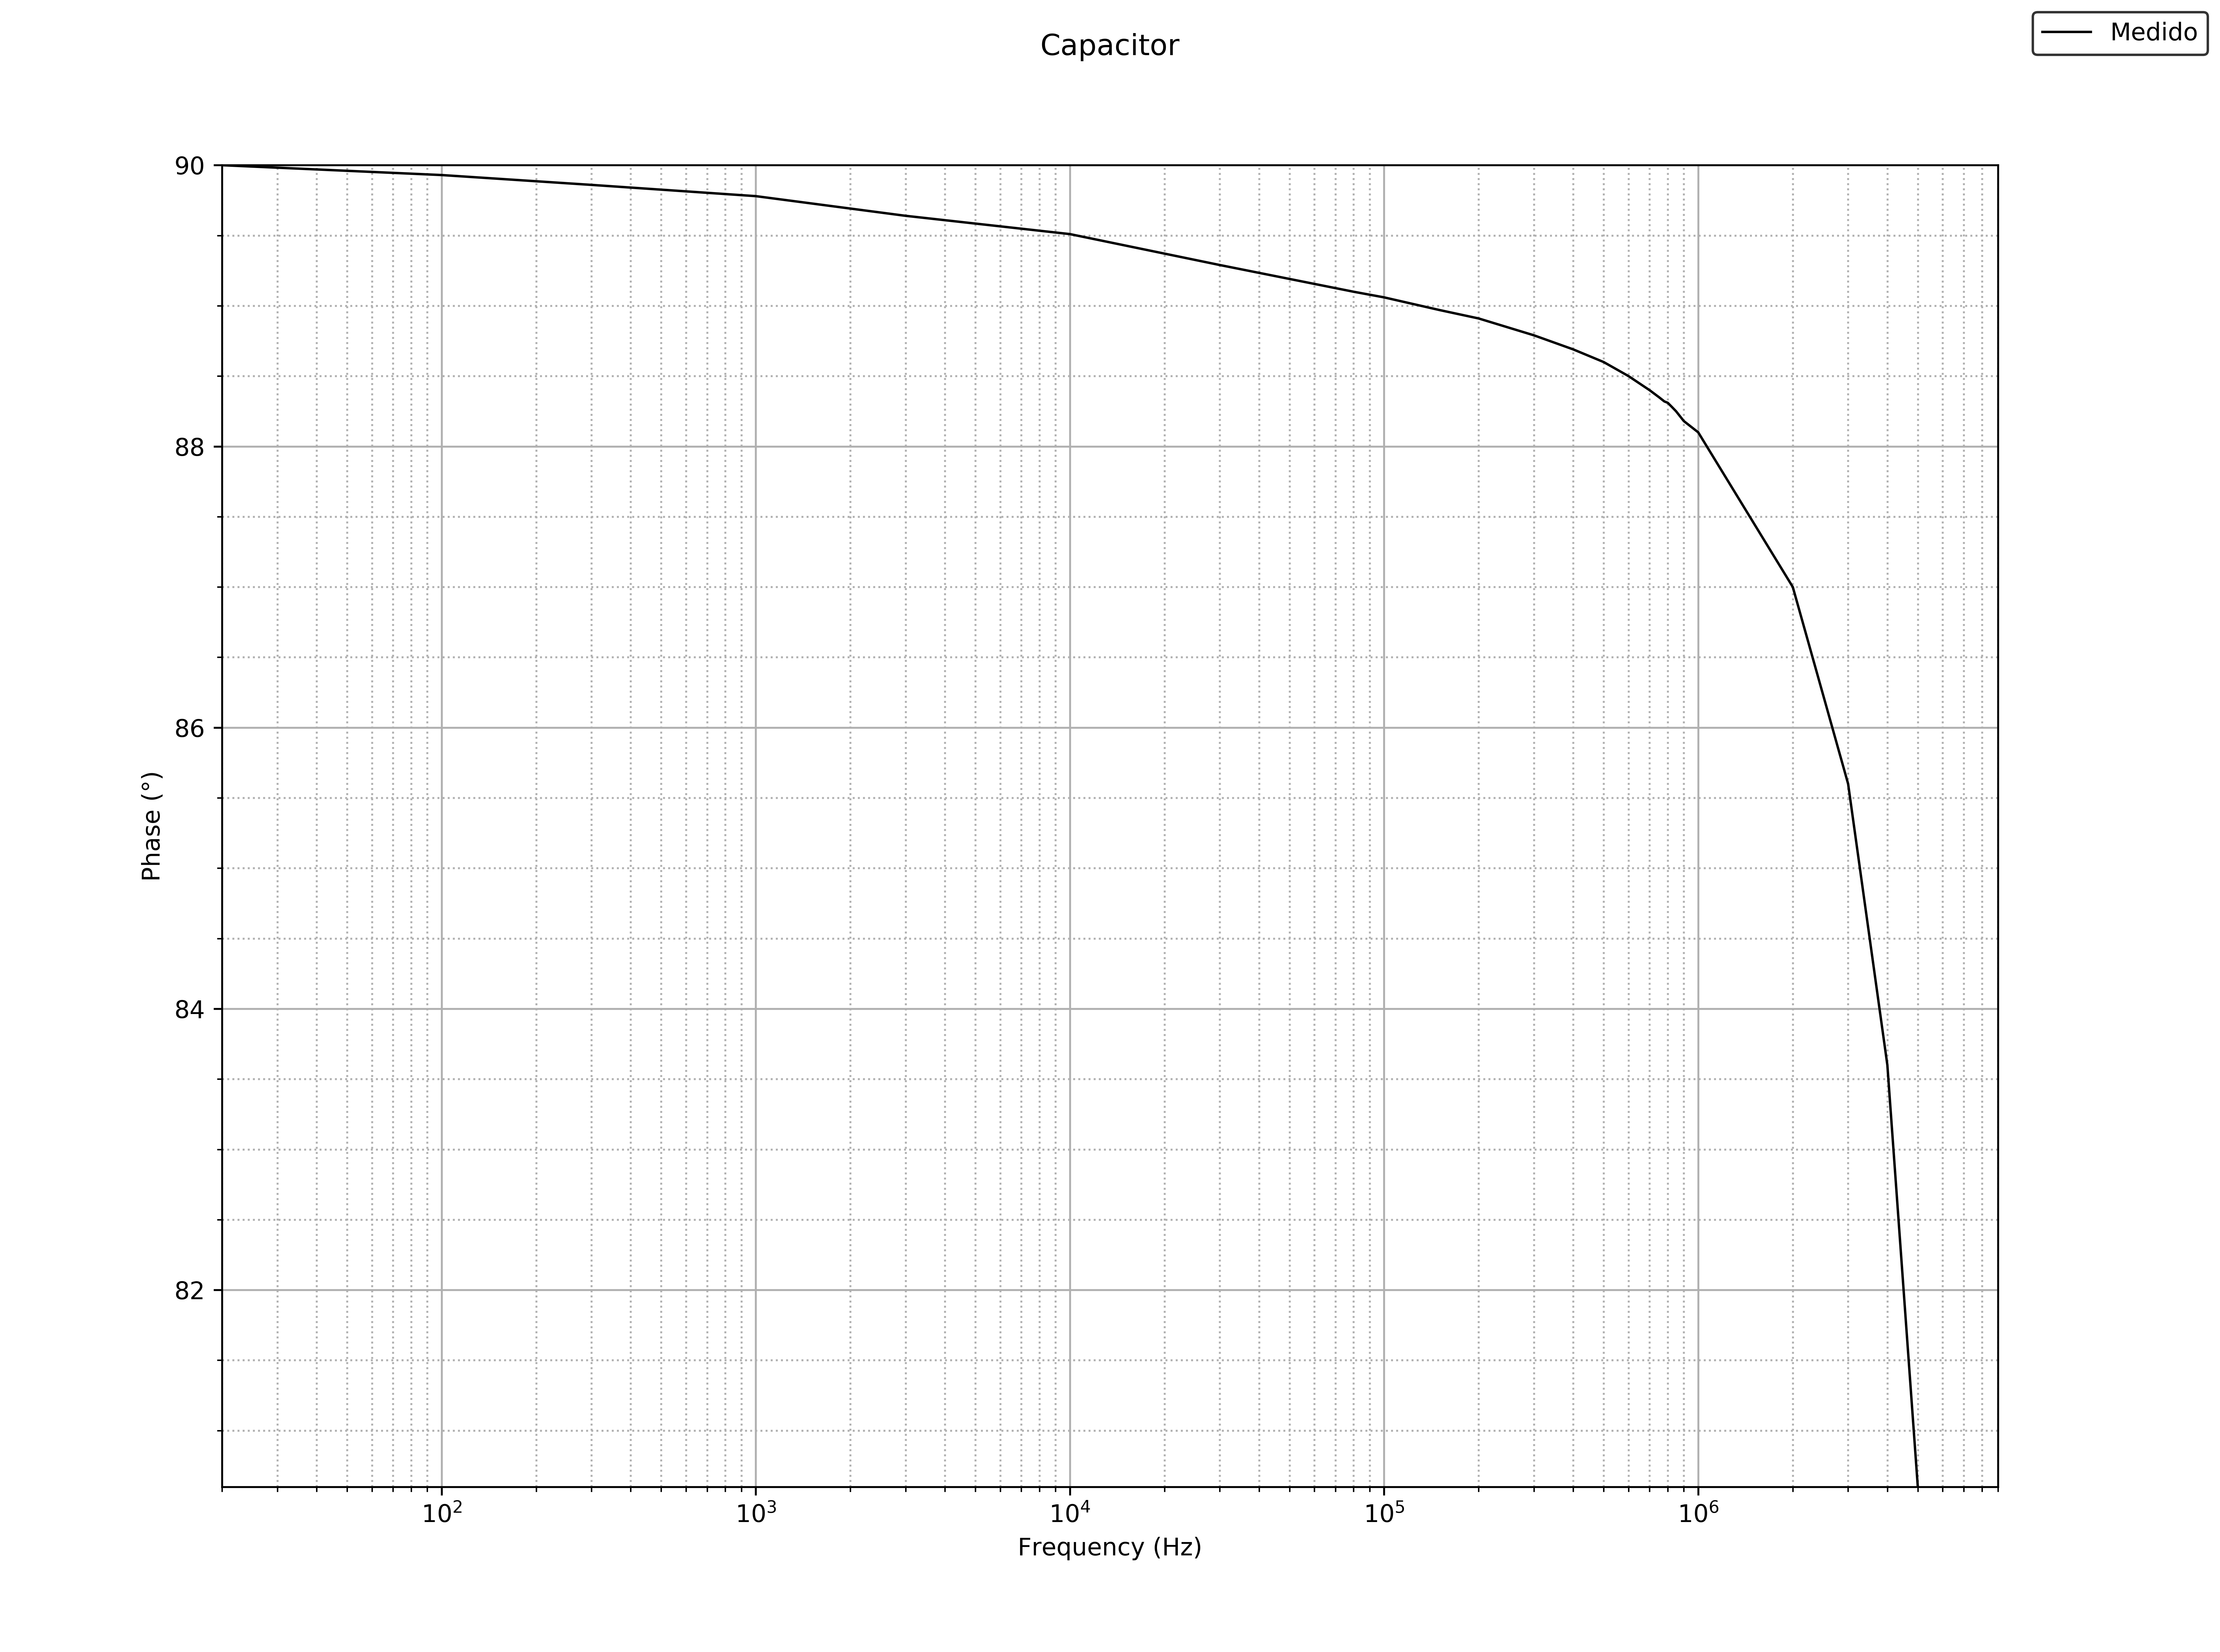
\includegraphics{Recursos/fase_medida_cap.png}

        \end{tabular}
    }
    \caption{Gr\'aficos realizados a partir de las mediciones}
    \label{fig:Med_CAP}
    
\end{figure}    


\subsubsection{Modelizaci\'on del comportamiento observado}
Se propone el circuito de la Figura \ref{fig:modelo_CAP} con el fin de encontrar un modelo que se ajuste al comportamiento real del capacitor tanto en impedancia como en fase.
\begin{figure}[H]
    \centering
    \resizebox{0.5\textwidth}{!}{
        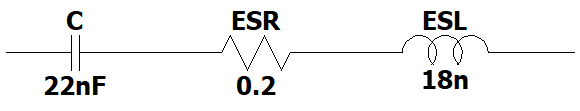
\includegraphics{Recursos/Modelo_cap.png}
    }
    \caption{Modelo de comportamiento del capacitor}
    \label{fig:modelo_CAP}
\end{figure}
El valor de la inductancia se parte de que la frecuencia de corte del sistema se encuentra en el punto donde el valor de capacidad arrojado por el analizador de impedancias pase de ser positivo a negativo, es decir, cuando el capacitor comienza a comportarse como un inductor. Del las mediciones se obtiene $f_{0} = 8MHz$. Luego, utilizando las f\'ormulas conocidas para un RLC serie mostradas en \ref{eq:RLC_CAP} y asumiendo que el valor de C es el nominal del componente utilizado.
\begin{equation}
    \omega_0 = \frac{1}{\sqrt{L \cdot C}} = 2 \cdot \pi \cdot f_0
    \label{eq:RLC_CAP}
\end{equation}
Resolviendo \ref{eq:RLC_CAP} se obtiene $L = 18nHy$.
Para ESR, se busca un valor iterando repetidas veces, hasta obtener una curva que se aproxime a la medida para la admitancia del capacitor.

Se muestran en la Figura \ref{fig:Comp_CAP}, los resultados obtenidos a partir del modelo elegido.

\begin{figure}[H]
    \centering
    \resizebox{\textwidth}{!}{
        \begin{tabular}{c c}
            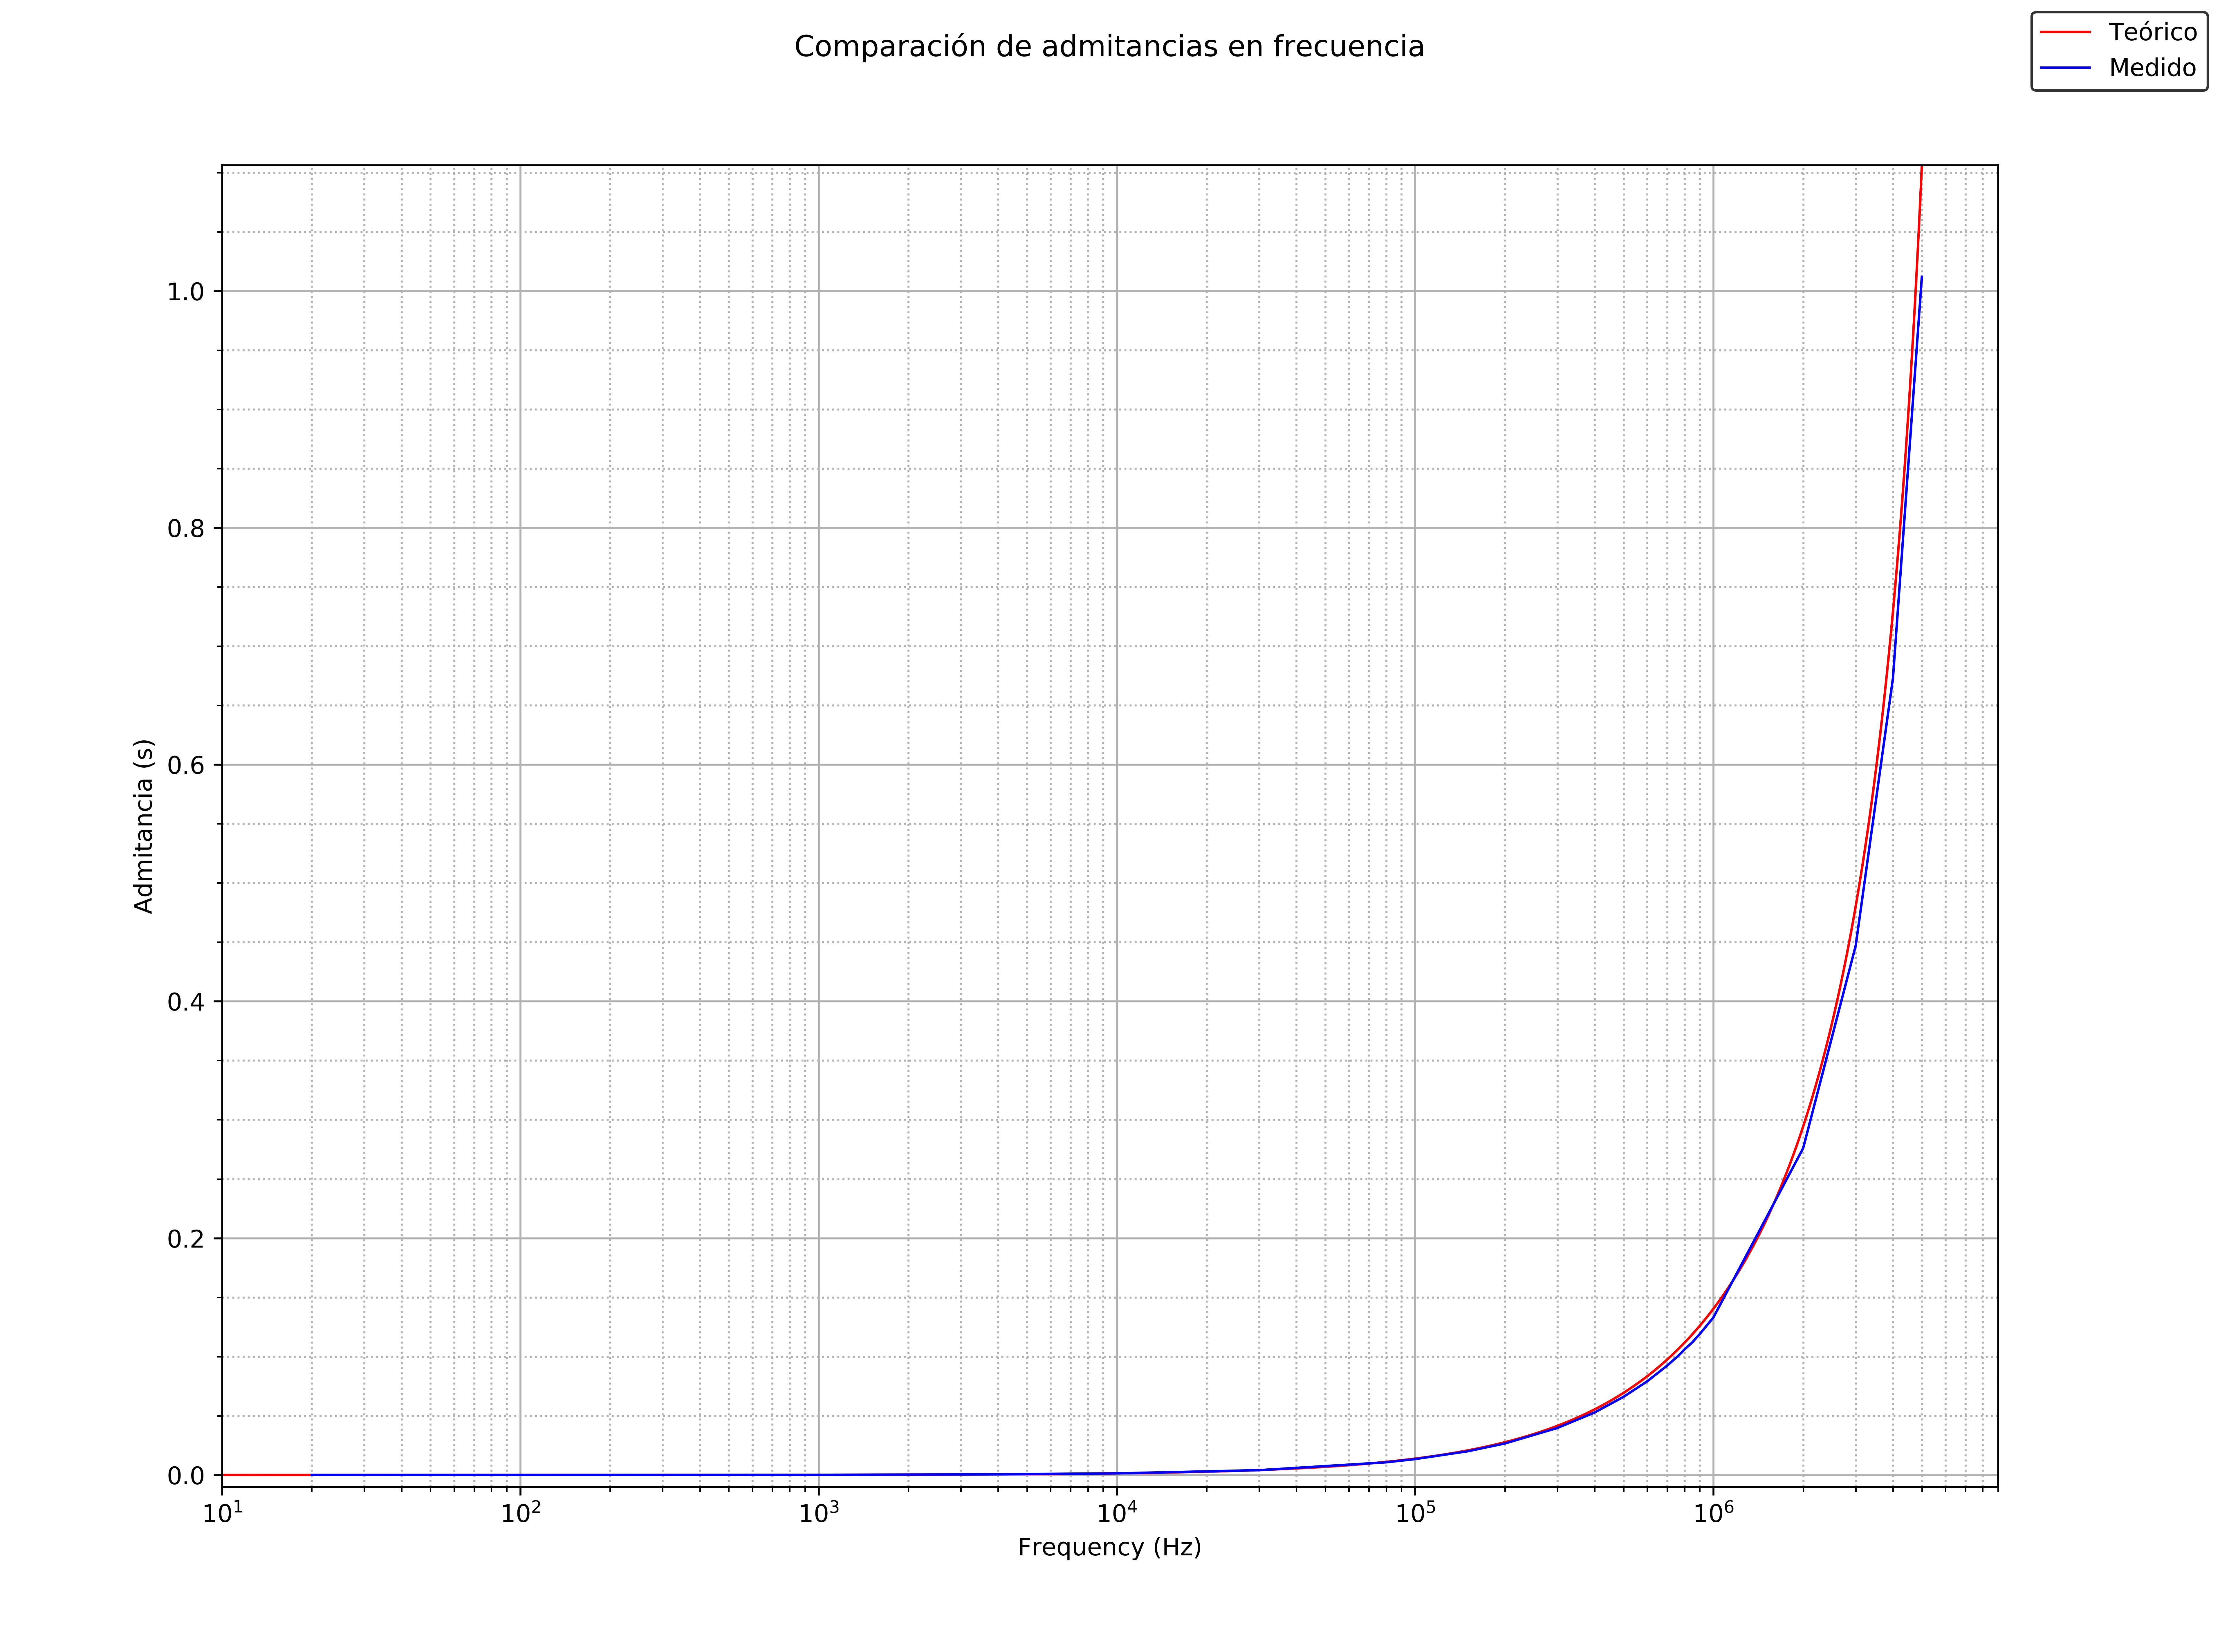
\includegraphics{Recursos/comp_admitancia_cap.png} &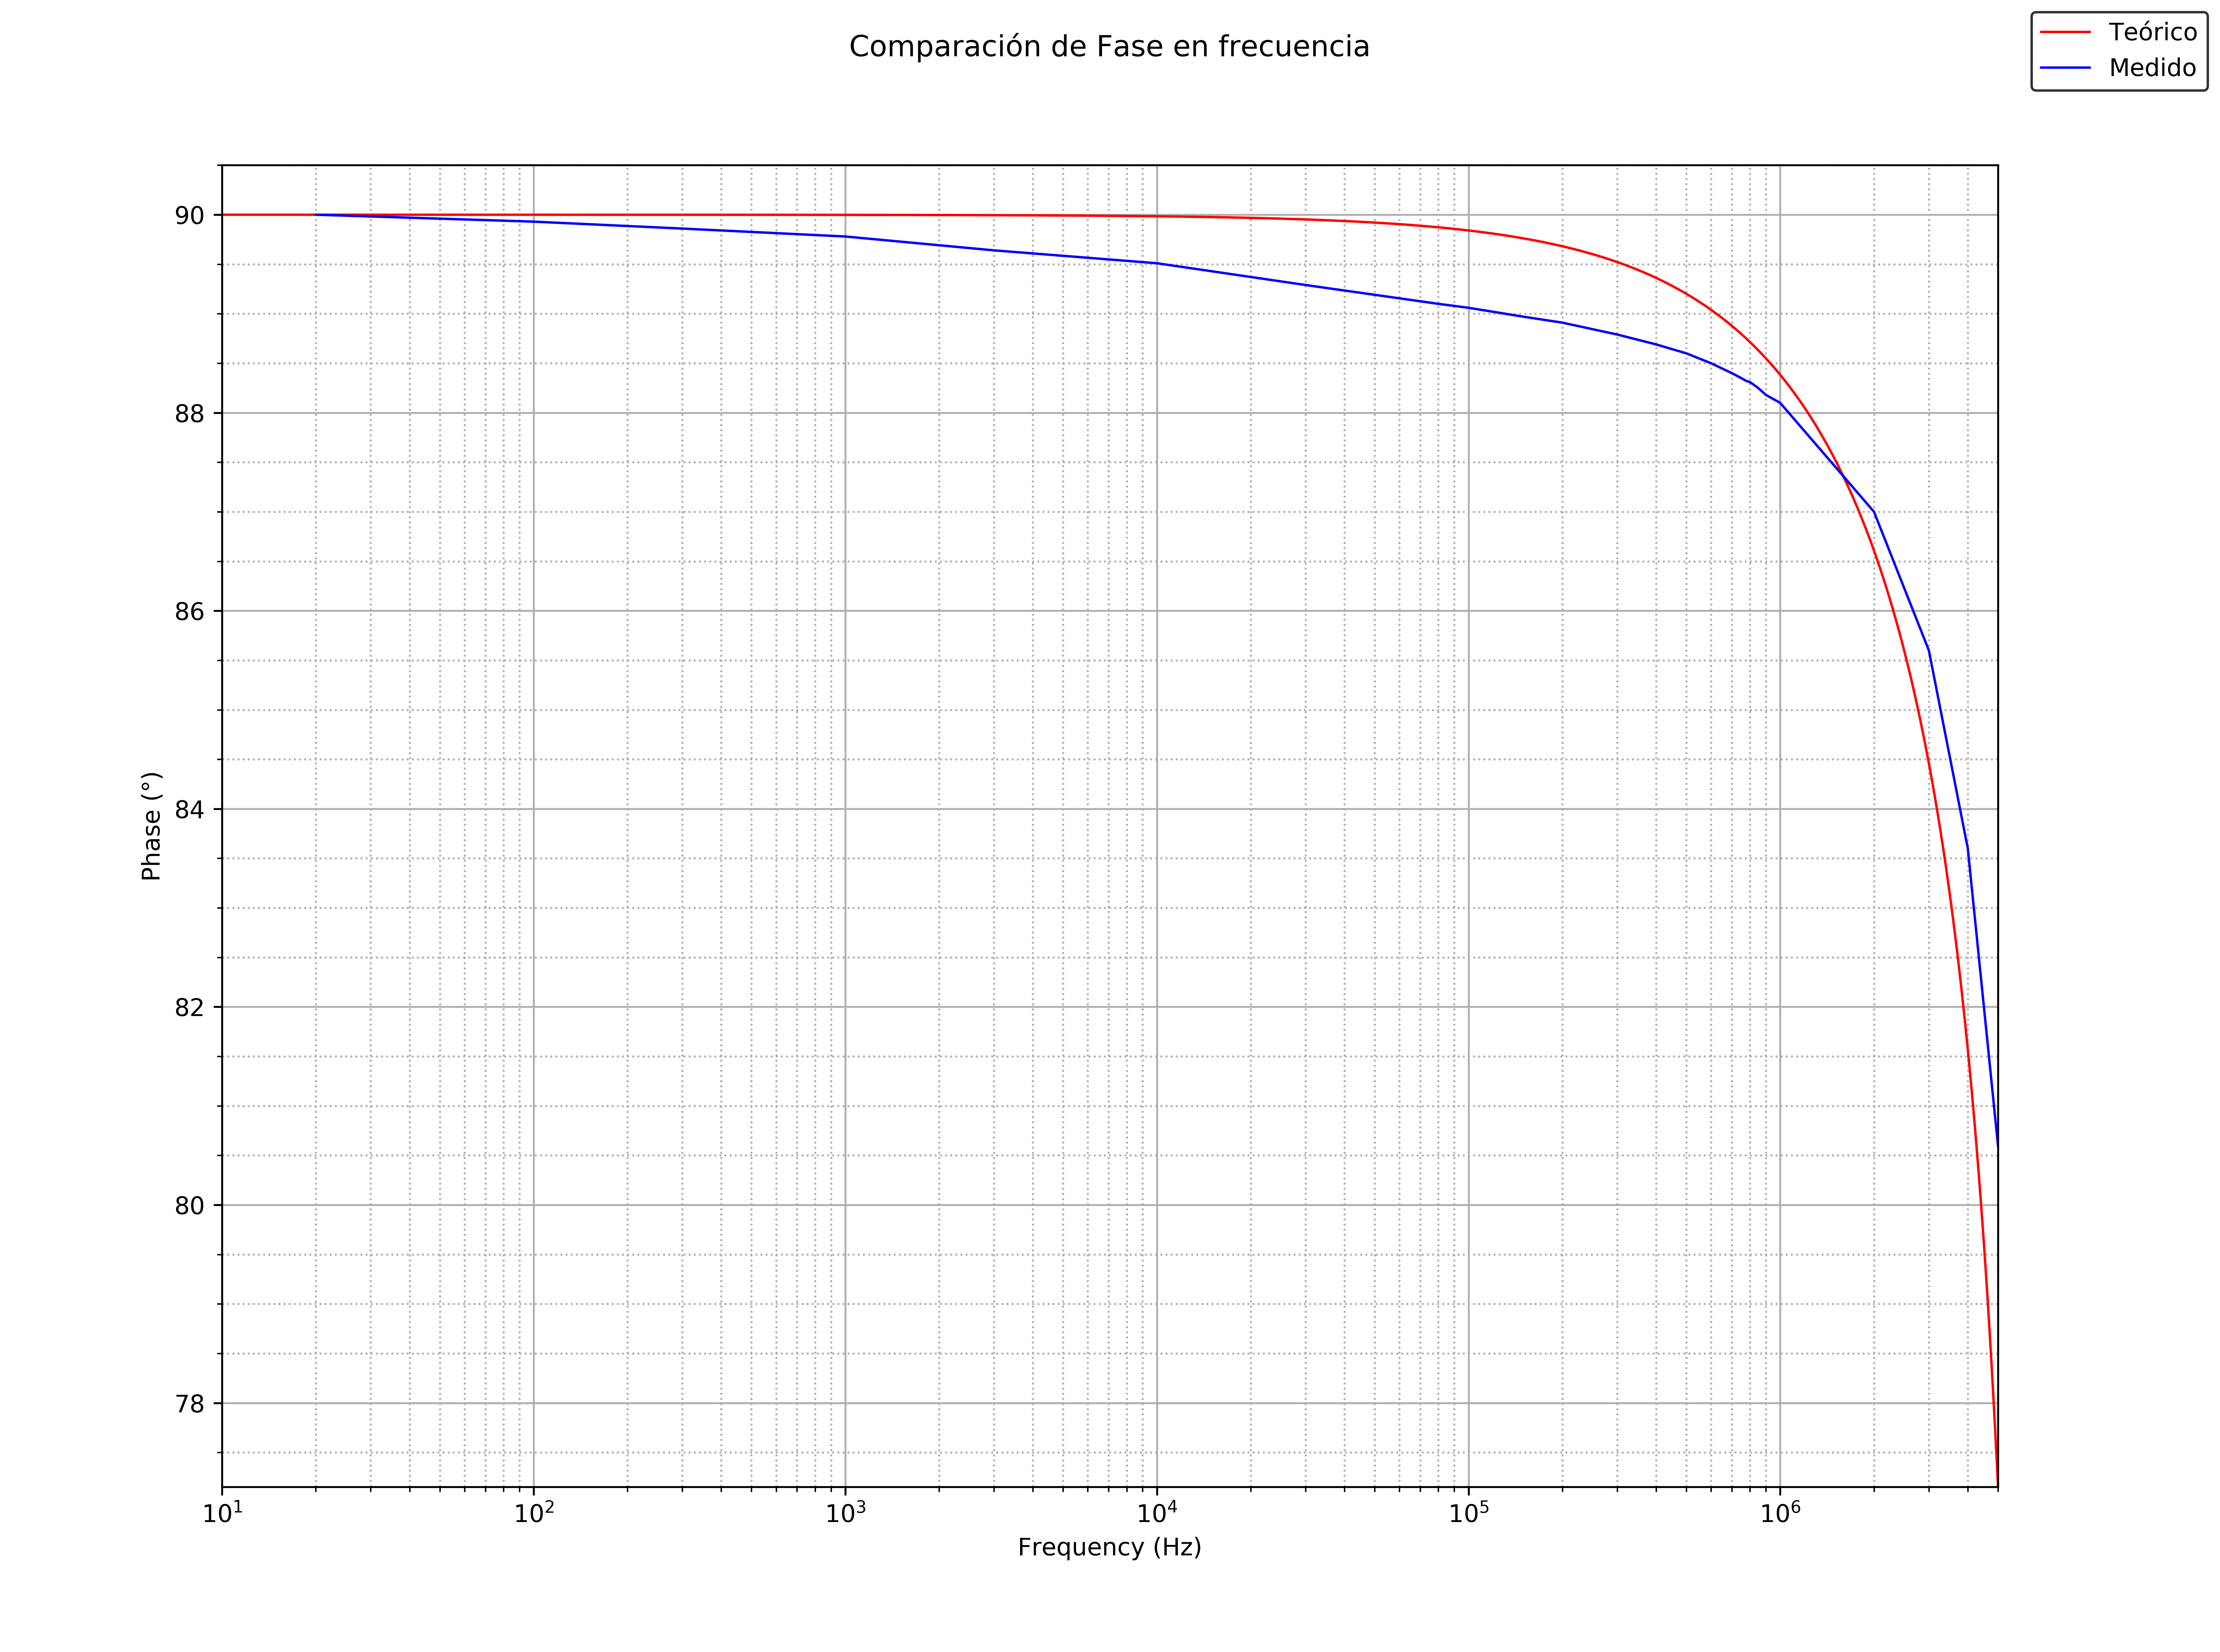
\includegraphics{Recursos/comp_fase_cap.png}
        \end{tabular}
        
    }
    \caption{Comparaci\'on entre mediciones y modelo de admitancia y fase en funci\'on de la frecuencia. }
        \label{fig:Comp_CAP}    
\end{figure}
Se observa un ajuste correcto en la comparaci\'on del modelo con las mediciones en el caso de la admitancia, lo que se corresponde con lo esperado ya que se dise\~na el circuito con ese fin. 

Si bien el comportamiento de la fase no coincide exactamente con el modelo, se puede observar que la forma es correcta. Se asume que estas diferencias son causadas por fen\'omenos no analizados en el capacitor como por ejemplo la variaci\'on de los valores de ESR y ESL con la frecuencia.

\subsection{Medici\'on del inductor}
Para la medici\'on se utiliza un inductor de $500\mu H$ con n\'ucleo de ferrite y se configura el analizador de impedancias en modelo serie para medir fase e impedancia. 
\subsubsection{Resultados}
Se muestran en la Tabla \ref{tab:Med_IND}  los resultados obtenidos de las mediciones y en la Figura \ref{fig:Med_IND} los respectivos  gr\'aficos realizados a partir de estas.
\begin{table}[H]
    \centering
    \resizebox{0.5\textwidth}{!}{%
        \begin{tabular}{ccccc}
            \hline
            \begin{tabular}[c]{@{}c@{}}Frecuencia\\   (Hz)
            \end{tabular} & Inductancia (Hy) & \begin{tabular}[c]{@{}c@{}}Factor de\\   calidad (Q)\end{tabular} & \multicolumn{1}{l}{Impedancia ($\Omega$)} & Fase ($^\circ$) \\ \hline
            10 & 5.00E-04 & 0 & 0.1 & 18.2 \\
            20 & 4.90E-04 & 1 & 1.13E-01 & 33 \\
            100 & 4.96E-04 & 3 & 0.328 & 71.6 \\
            300 & 4.92E-04 & 8 & 9.35E-01 & 82.6 \\
            1000 & 4.94E-04 & 16 & 3.11 & 86.4 \\
            3000 & 4.89E-04 & 23.5 & 9.23E+00 & 87.54 \\
            10000 & 4.89E-04 & 25 & 30.77 & 87.67 \\
            30000 & 4.77E-04 & 22.5 & 9.02E+01 & 87.43 \\
            80000 & 4.64E-04 & 17 & 2.34E+02 & 86.6 \\
            100000 & 4.66E-04 & 14.7 & 293 & 86.09 \\
            150000 & 4.66E-04 & 11.3 & 4.41E+02 & 84.93 \\
            200000 & 4.73E-04 & 8.9 & 5.98E+02 & 83.57 \\
            300000 & 5.00E-04 & 5.9 & 9.56E+02 & 80.47 \\
            400000 & 5.47E-04 & 4.1 & 1.41E+03 & 76.42 \\
            500000 & 6.20E-04 & 2.9 & 2.06E+03 & 70.7 \\
            600000 & 7.15E-04 & 1.8 & 3.07E+03 & 61.5 \\
            700000 & 7.52E-04 & 1 & 4.73E+03 & 44.4 \\
            750000 & 6.18E-04 & 0.6 & 5.80E+03 & 30.24 \\
            780000 & 4.32E-04 & 0.4 & 6.37E+03 & 19.4 \\
            800000 & 2.56E-04 & 0.2 & 6.66E+03 & 11.11 \\
            825000 & 2.30E-05 & 0 & 6.84E+03 & 1.04 \\
            850000 & -2.05E-04 & 0.2 & 6.78E+03 & -9.29 \\
            875000 & -3.80E-04 & 0.3 & 6.54E+03 & -18.86 \\
            900000 & -5.03E-04 & 0.5 & 6.16E+03 & -27.5 \\
            950000 & -5.82E-04 & 0.9 & 5.31E+03 & -40.89 \\
            1000000 & -5.53E-04 & 1.2 & 4.48E+03 & -50.73 \\
            1250000 & -2.90E-04 & 2.8 & 2.47E+03 & -70.5 \\
            1500000 & -1.70E-04 & 4.4 & 1.71E+03 & -77.11 \\
            1650000 & -1.38E-04 & 5.3 & 1.46E+03 & -79.25 \\
            1750000 & -1.19E-04 & 5.8 & 1.33E+03 & -80.31 \\
            2000000 & -8.59E-05 & 7.3 & 1.08E+03 & -82.24 \\
            3000000 & -3.43E-05 & 12.8 & 6.48E+02 & -85.51 \\
            4000000 & -1.86E-05 & 17.5 & 4.66E+02 & -86.7 \\
            5000000 & -1.16E-05 & 21.2 & 3.65E+02 & -87.27 \\
            10000000 & -2.70E-06 & 24.6 & 170.4 & -87.64 \\ \hline
        \end{tabular}%
    }
    \caption{Mediciones del inductor}
    \label{tab:Med_IND}
\end{table}
\begin{figure}[H]
    \centering
    \resizebox{\textwidth}{!}{
        \begin{tabular}{c c}
            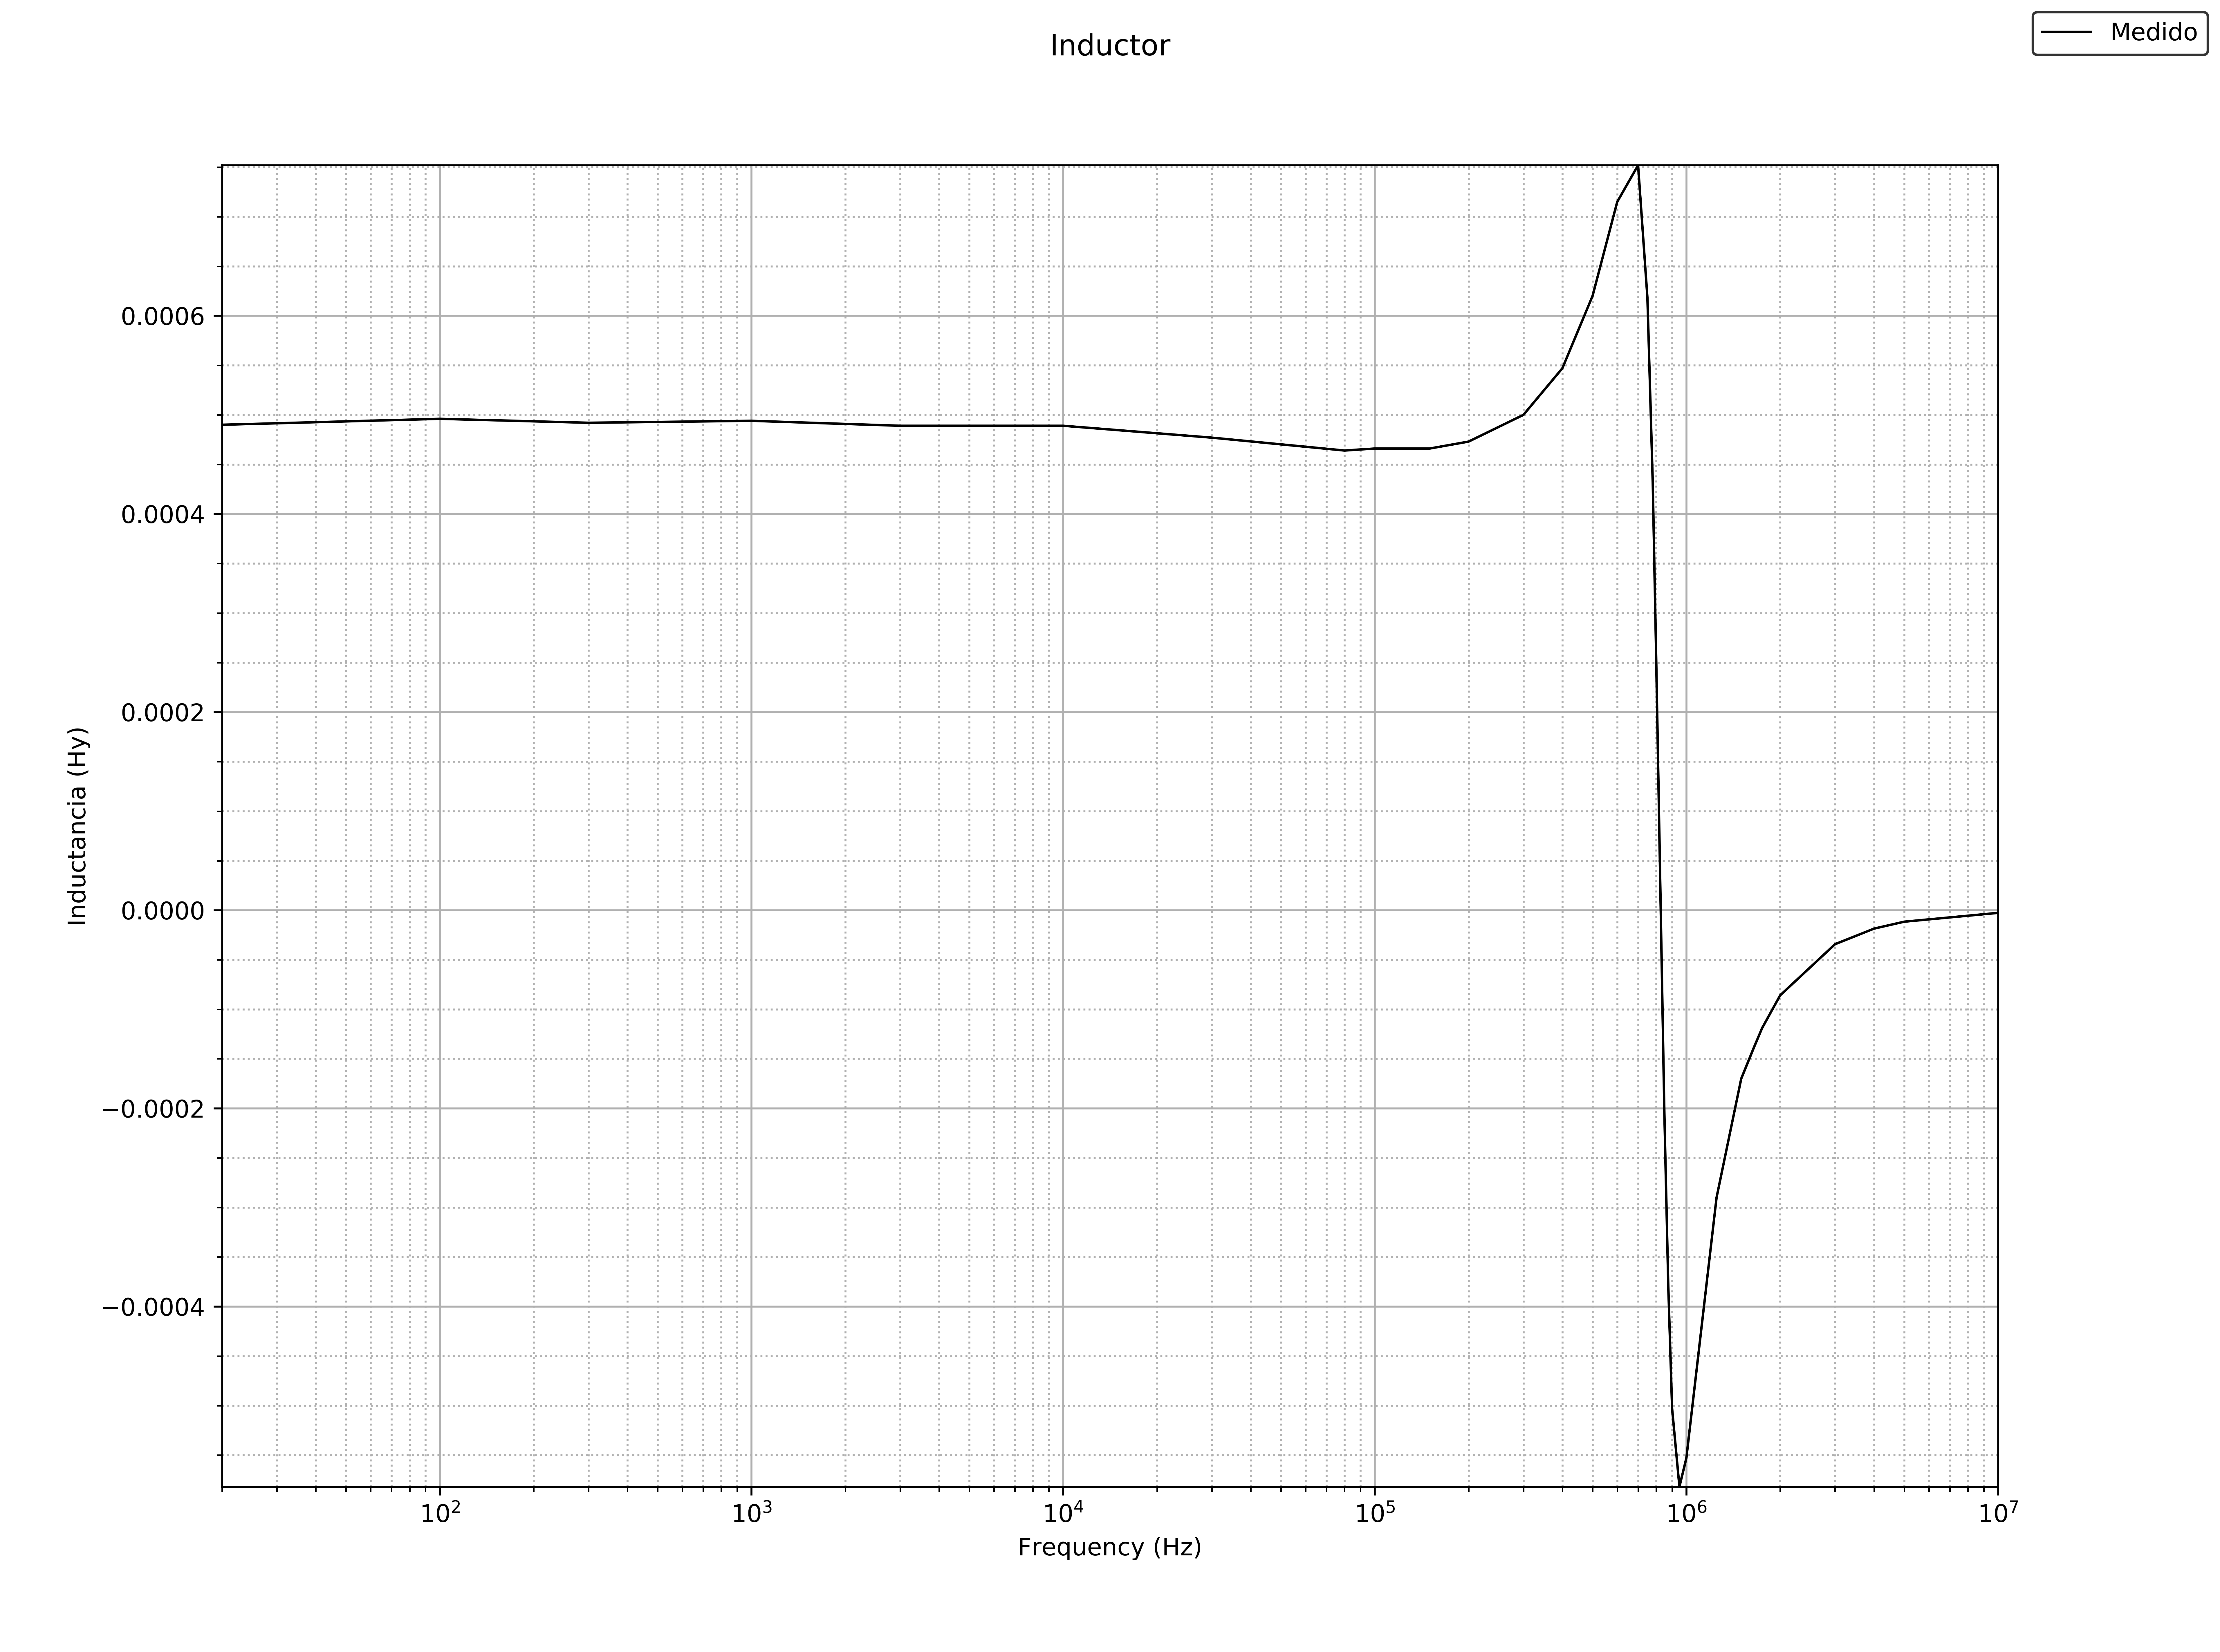
\includegraphics{Recursos/inductancia_medida_ind.png}&
            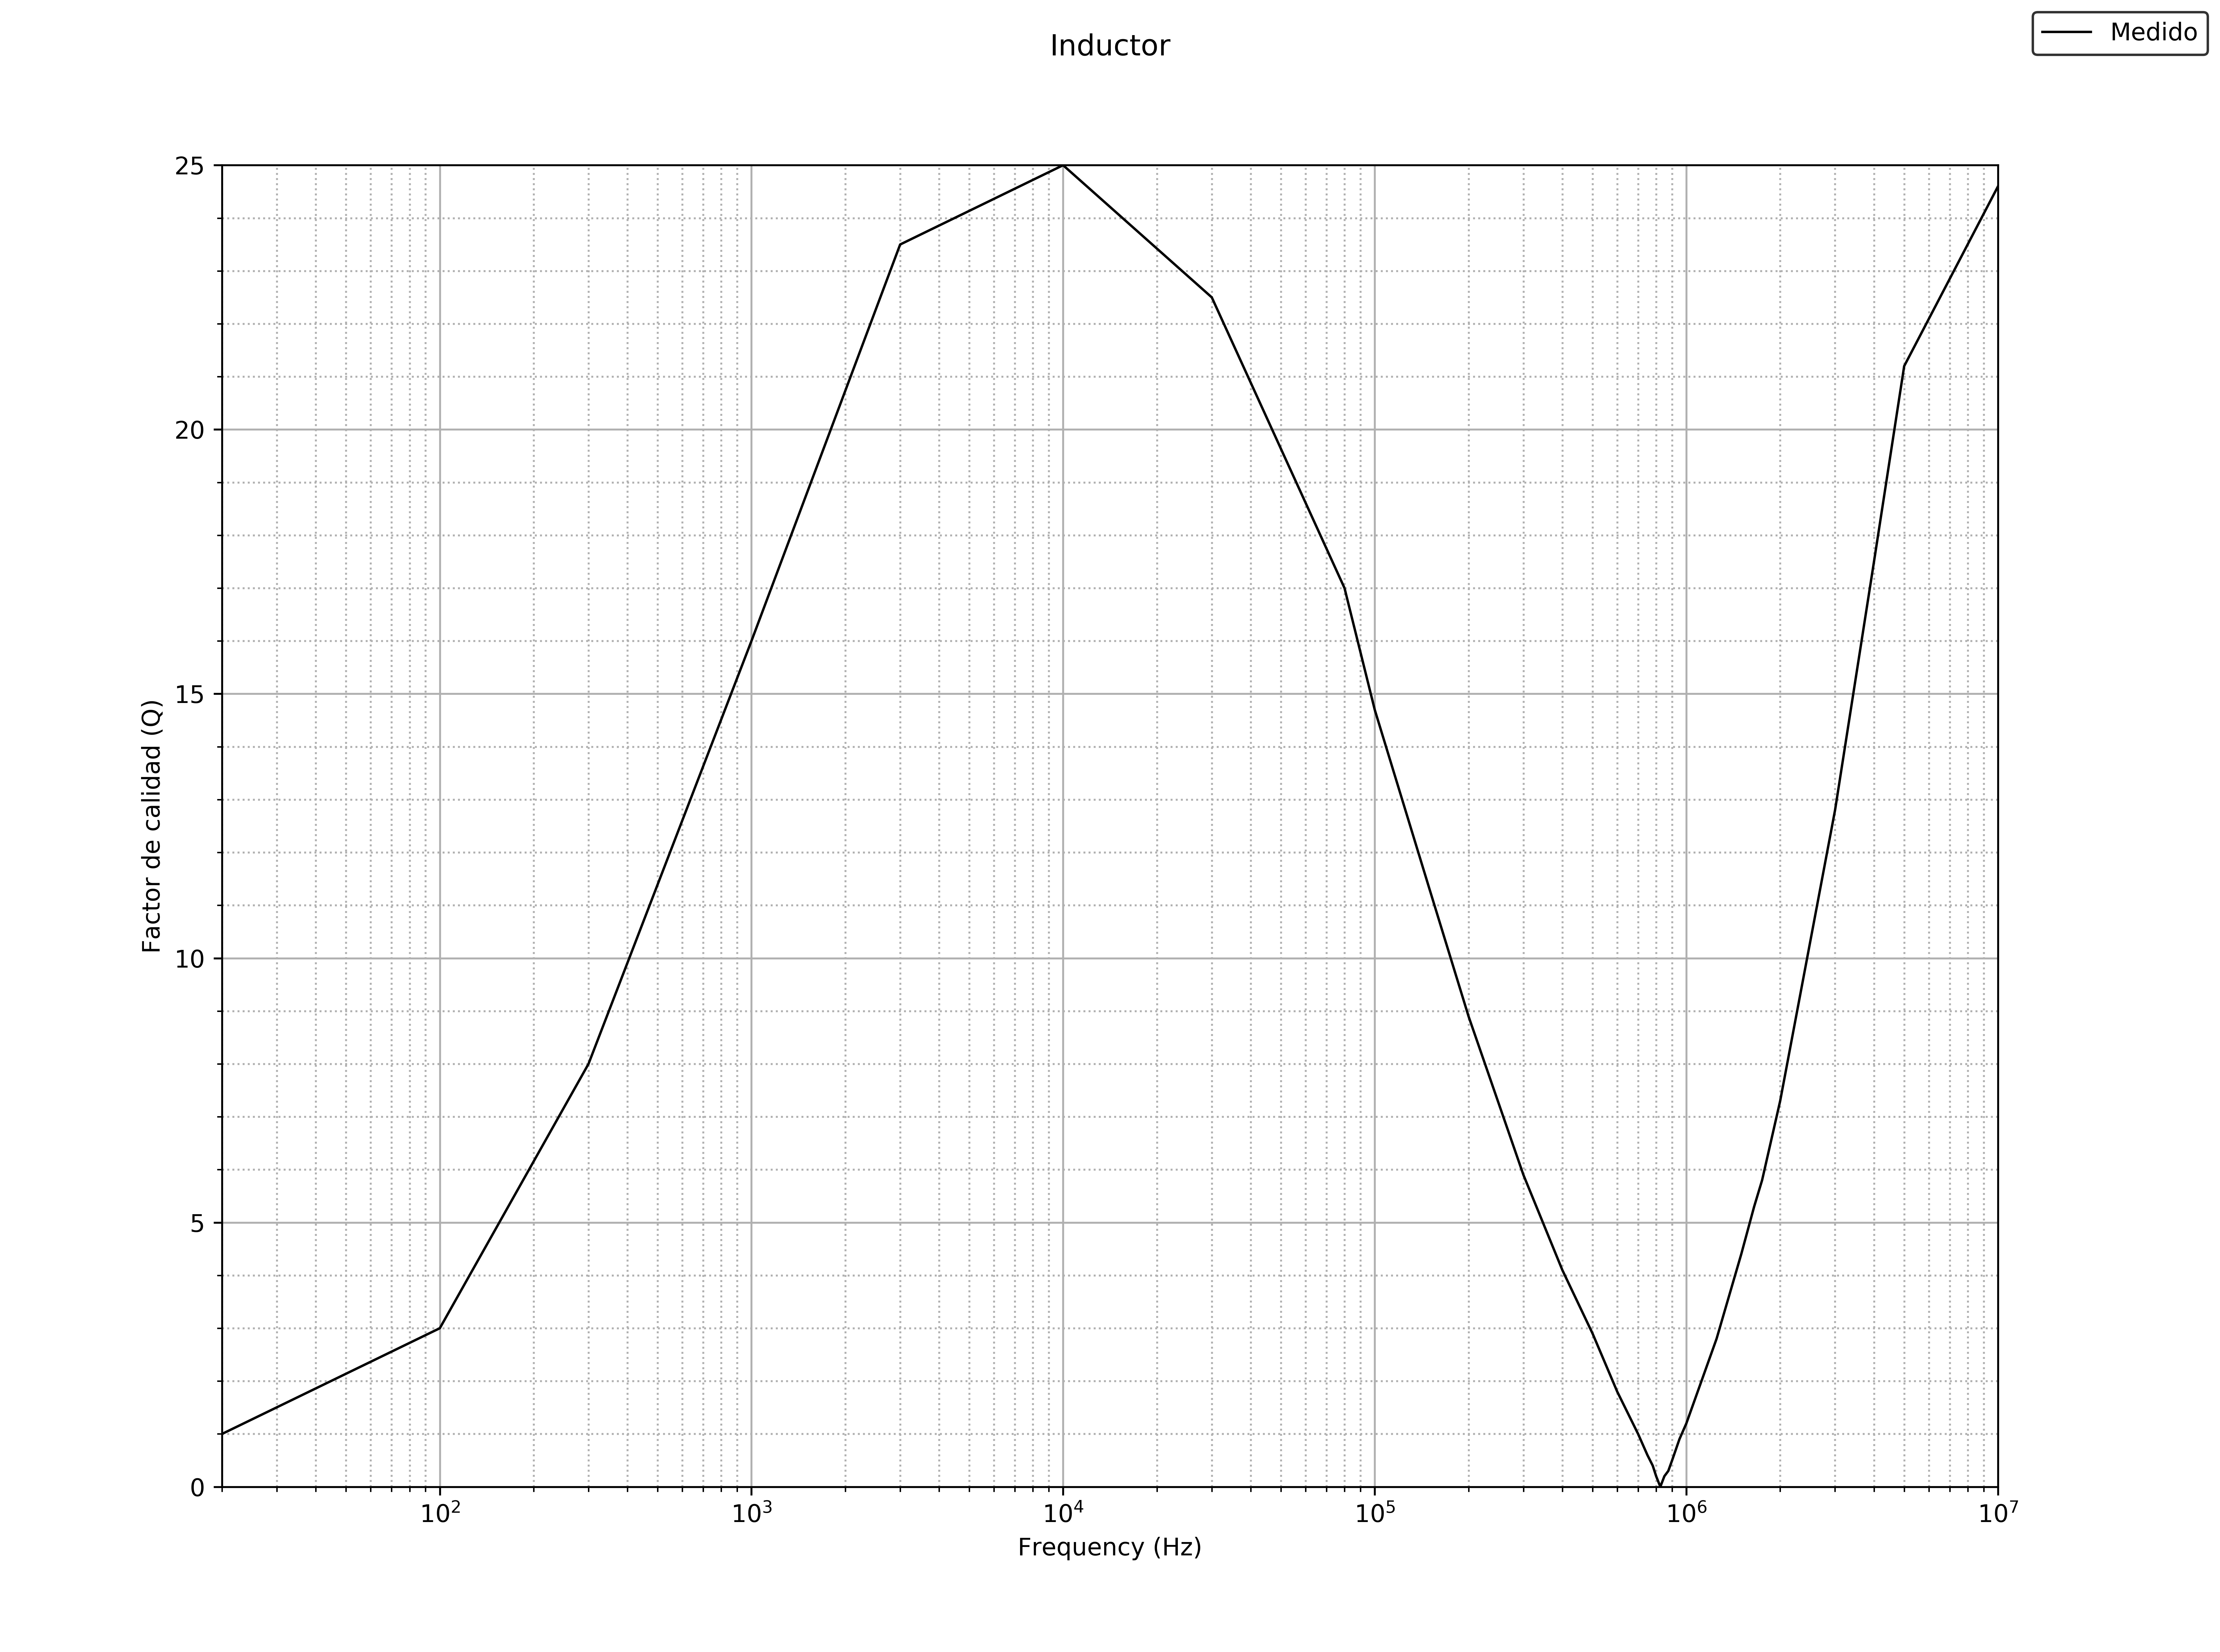
\includegraphics{Recursos/calidad_medida_ind.png} \\
            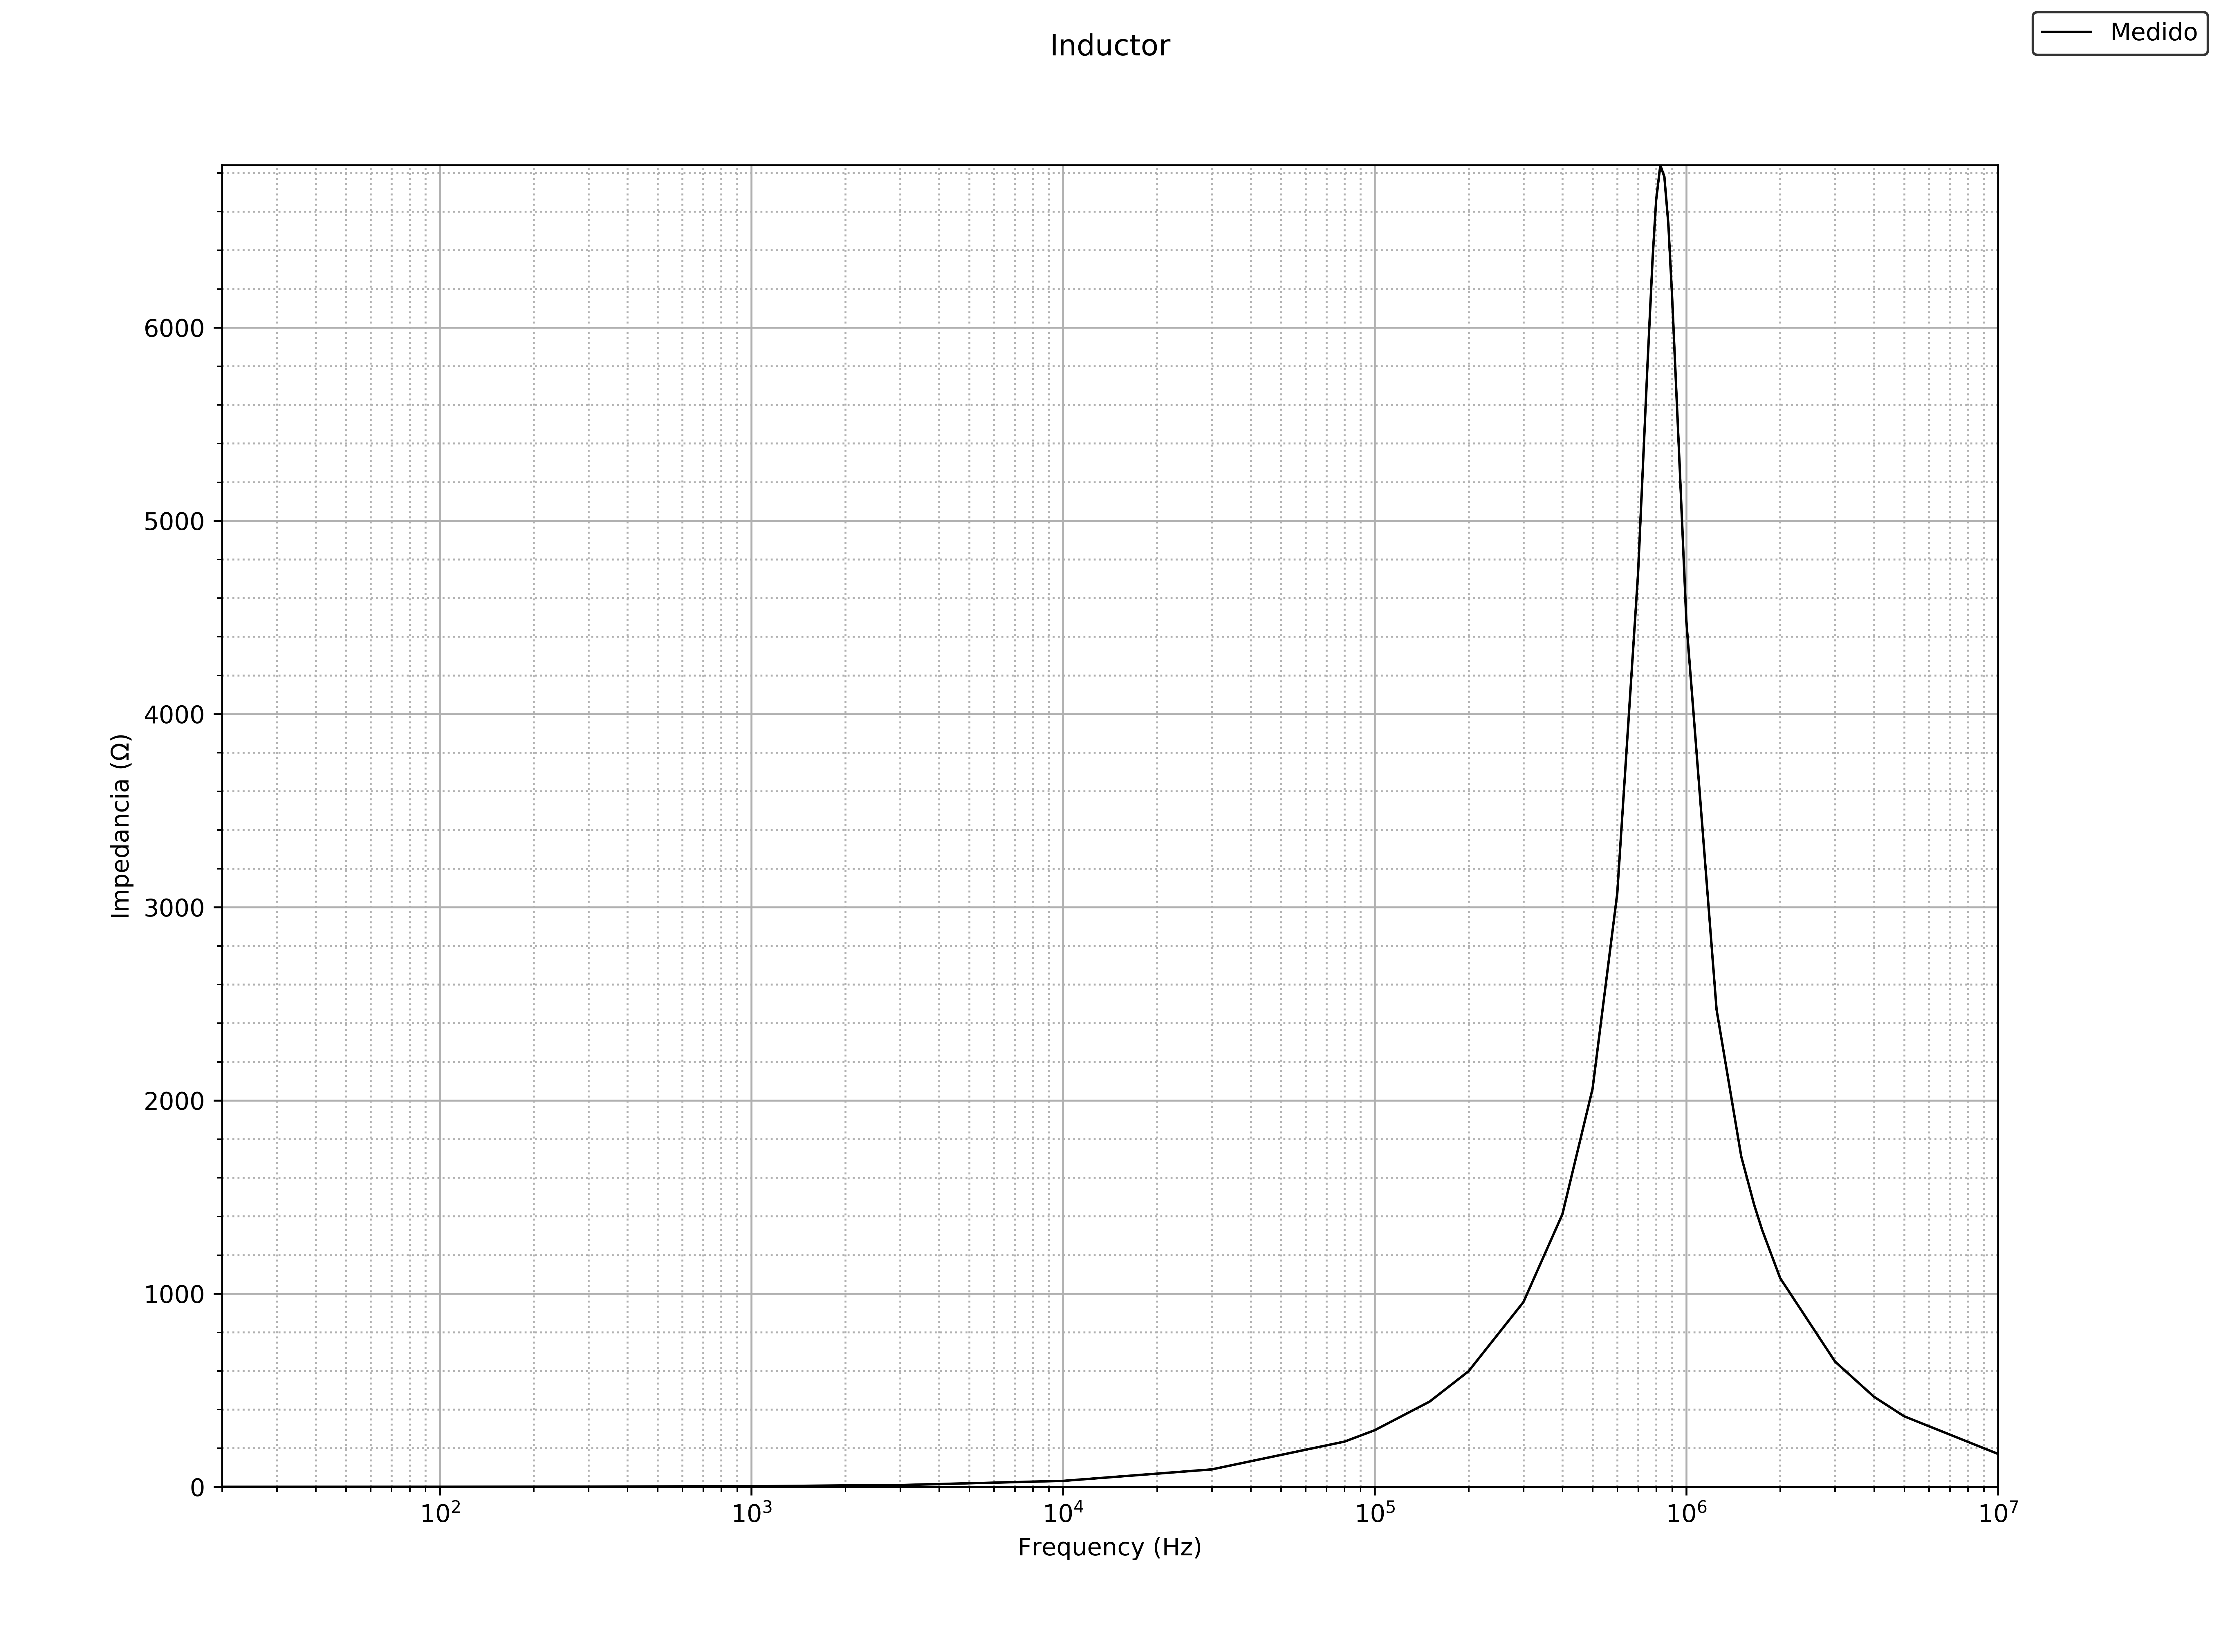
\includegraphics{Recursos/impedancia_medida_ind.png} &
            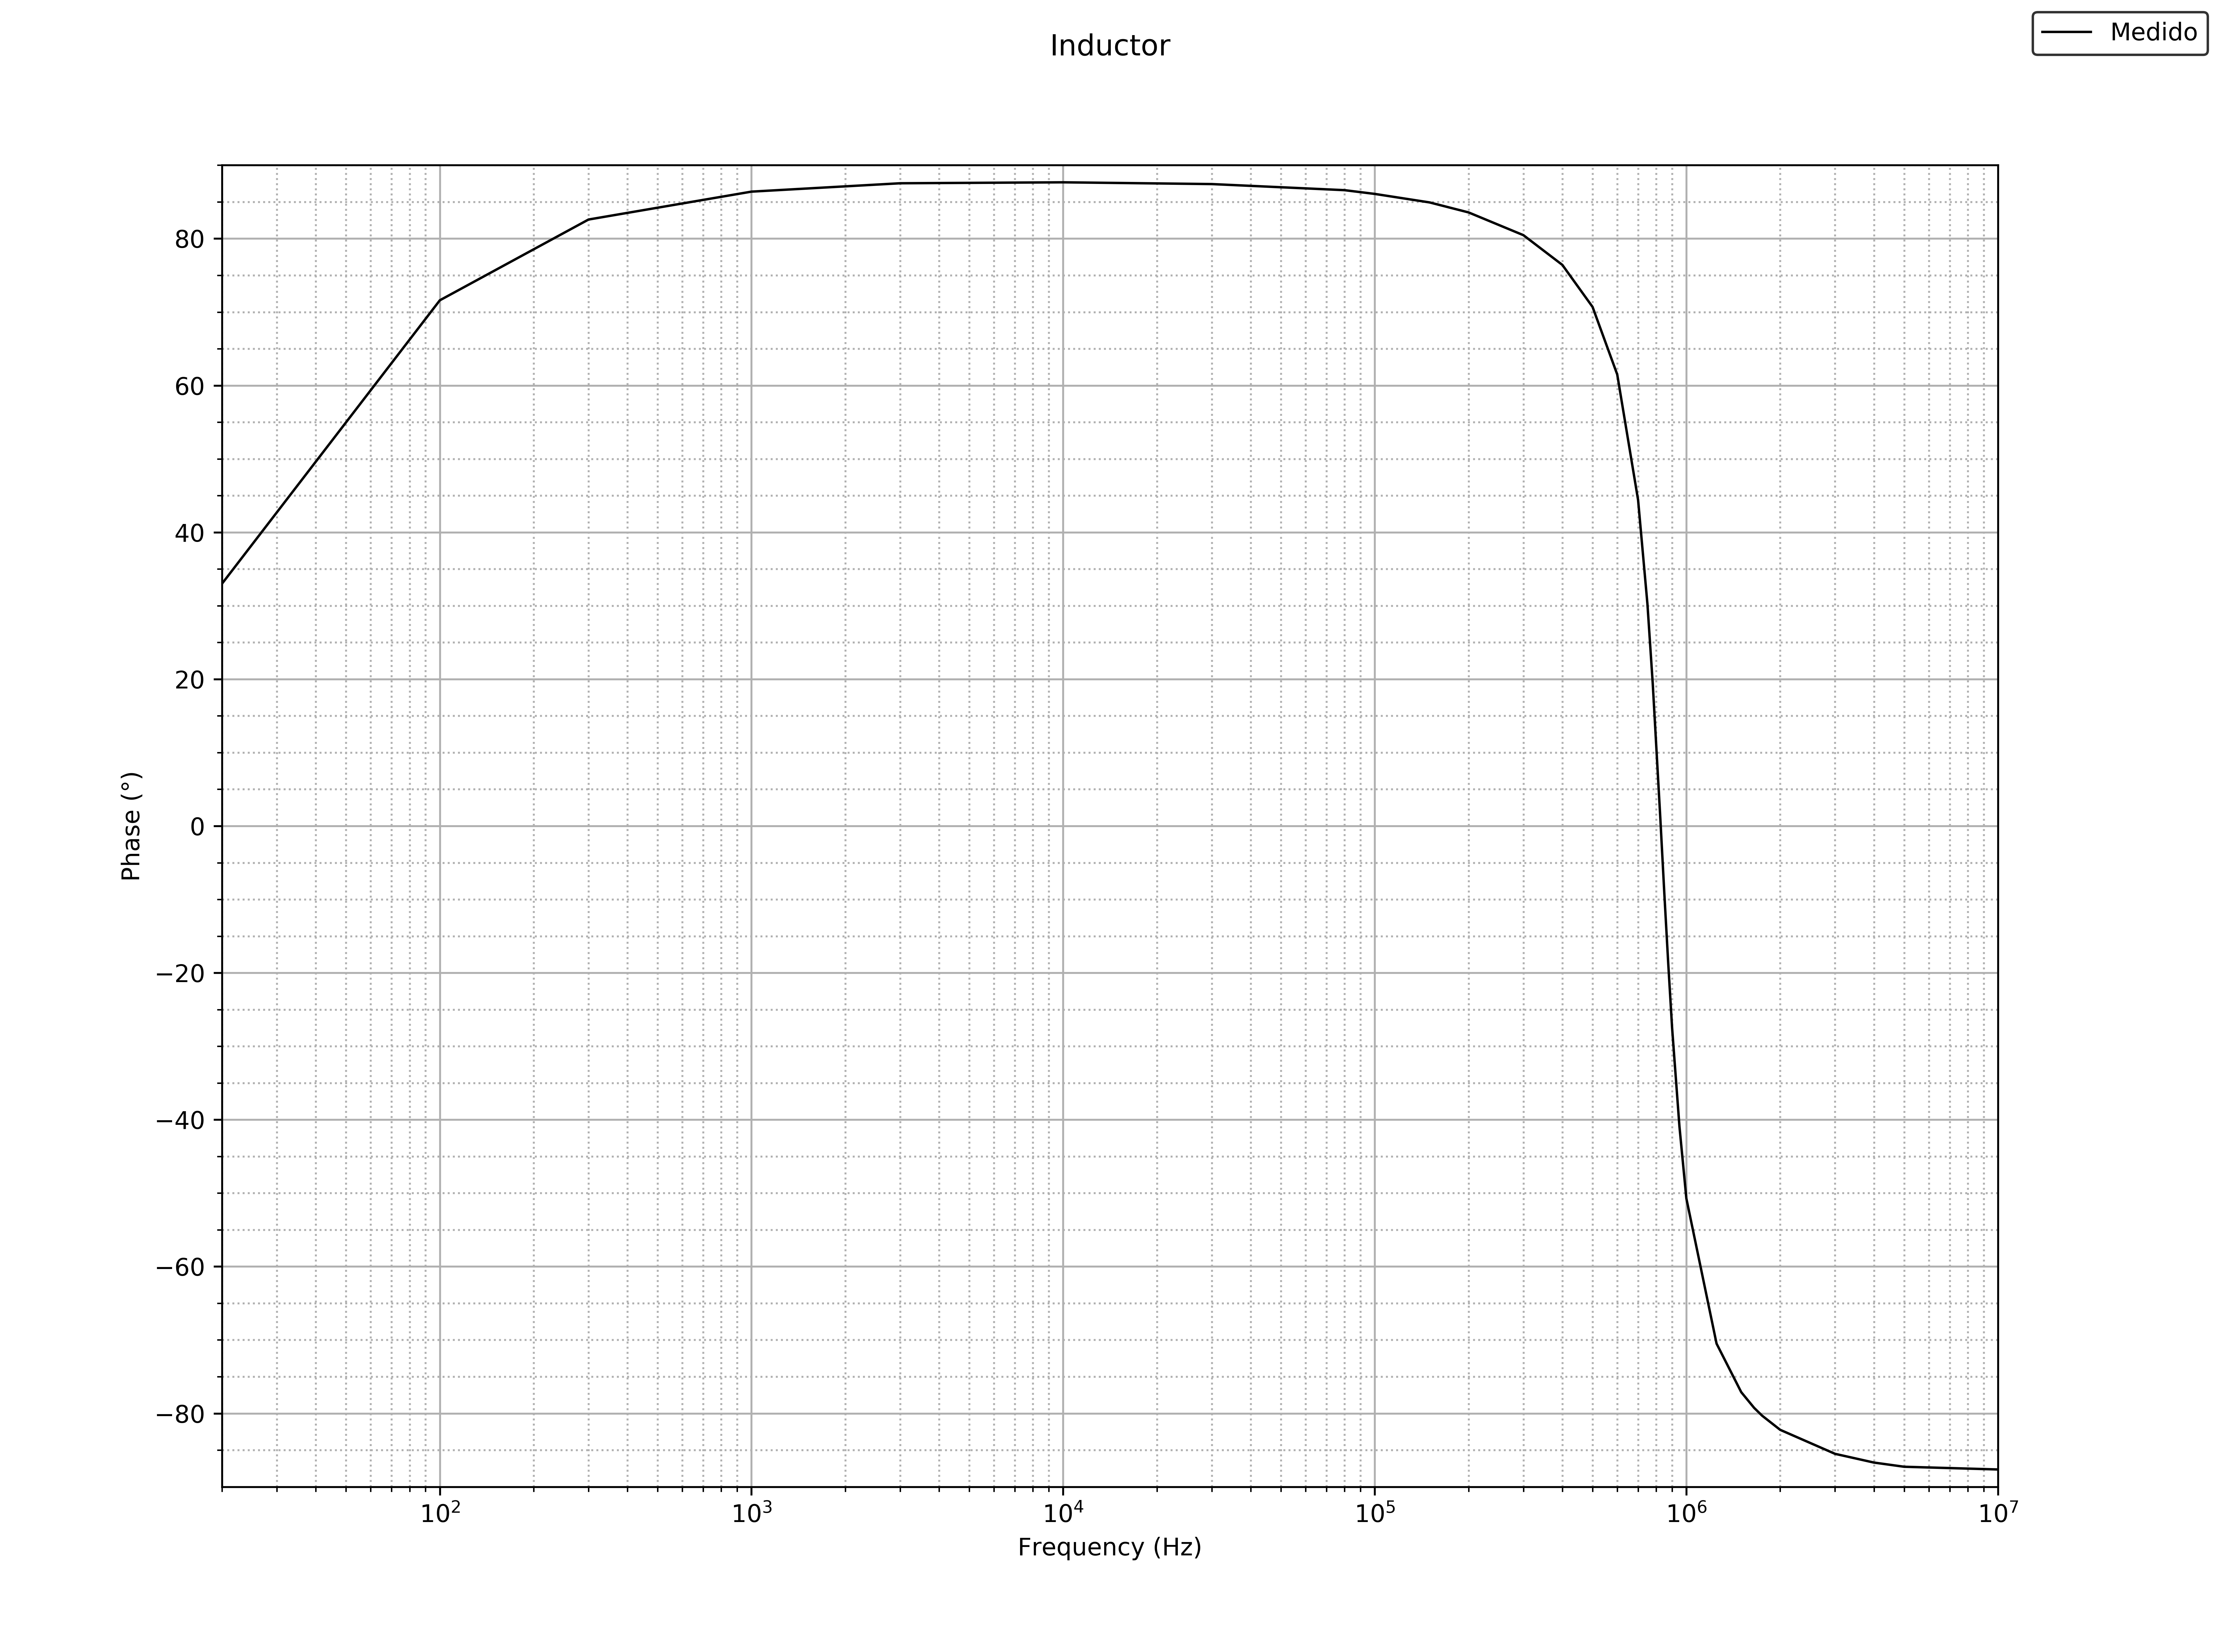
\includegraphics{Recursos/fase_medida_ind.png}

        \end{tabular}
    }
    \caption{Gr\'aficos realizados a partir de las mediciones}
    \label{fig:Med_IND}
        
\end{figure}    

\subsubsection{Modelizaci\'on del comportamiento observado}
Se propone el circuito de la Figura \ref{fig:modelo_IND} con el fin de encontrar un modelo que se ajuste al comportamiento real del inductor tanto en impedancia como en fase.
\begin{figure}[H]
    \centering
    \resizebox{0.5\textwidth}{!}{
        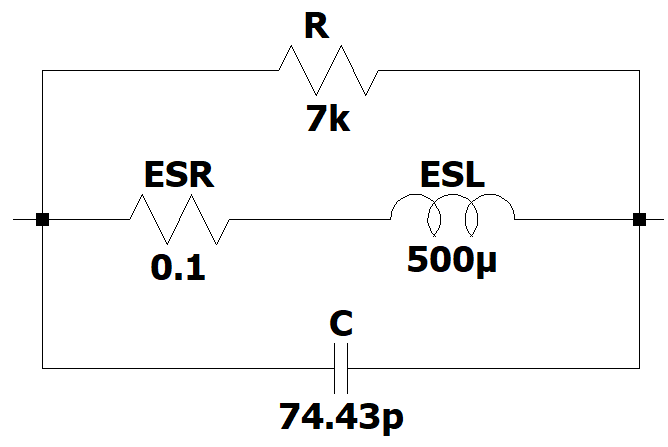
\includegraphics{Recursos/Modelo_ind.png}
    }
    \caption{Modelo de comportamiento del inductor}
    \label{fig:modelo_IND}
\end{figure}
Asumiendo que el valor de la inductancia es de $500\mu Hy$, lo cual es correcto si se tiene en cuanta que para frecuencias medias ese es el valor que se obtuvo en las mediciones, se puede encontrar un valor para $C$ de igual forma que para el modelo del capacitor y tomando el valor para la frecuencia de corte $f_0 = 825KHz$ que nuevamente es el valor para el cual la inductancia medida con el analizador de impedancias pasa de positiva a negativa.

Para los valores de $ESR$ y $R$ se eligen valores de manera que para frecuencias bajas la resistencia equivalente del modelo coincida con la impedancia medida, y se fija el valor $R = 7K\Omega$ para lograr un mejor ajuste a la curva medida, limitando la m\'axima impedancia del modelo.

Se muestran en la Figura \ref{fig:Comp_IND}, los resultados obtenidos a partir del modelo elegido.
\begin{figure}[H]
    \centering
    \resizebox{\textwidth}{!}{
        \begin{tabular}{c c}
            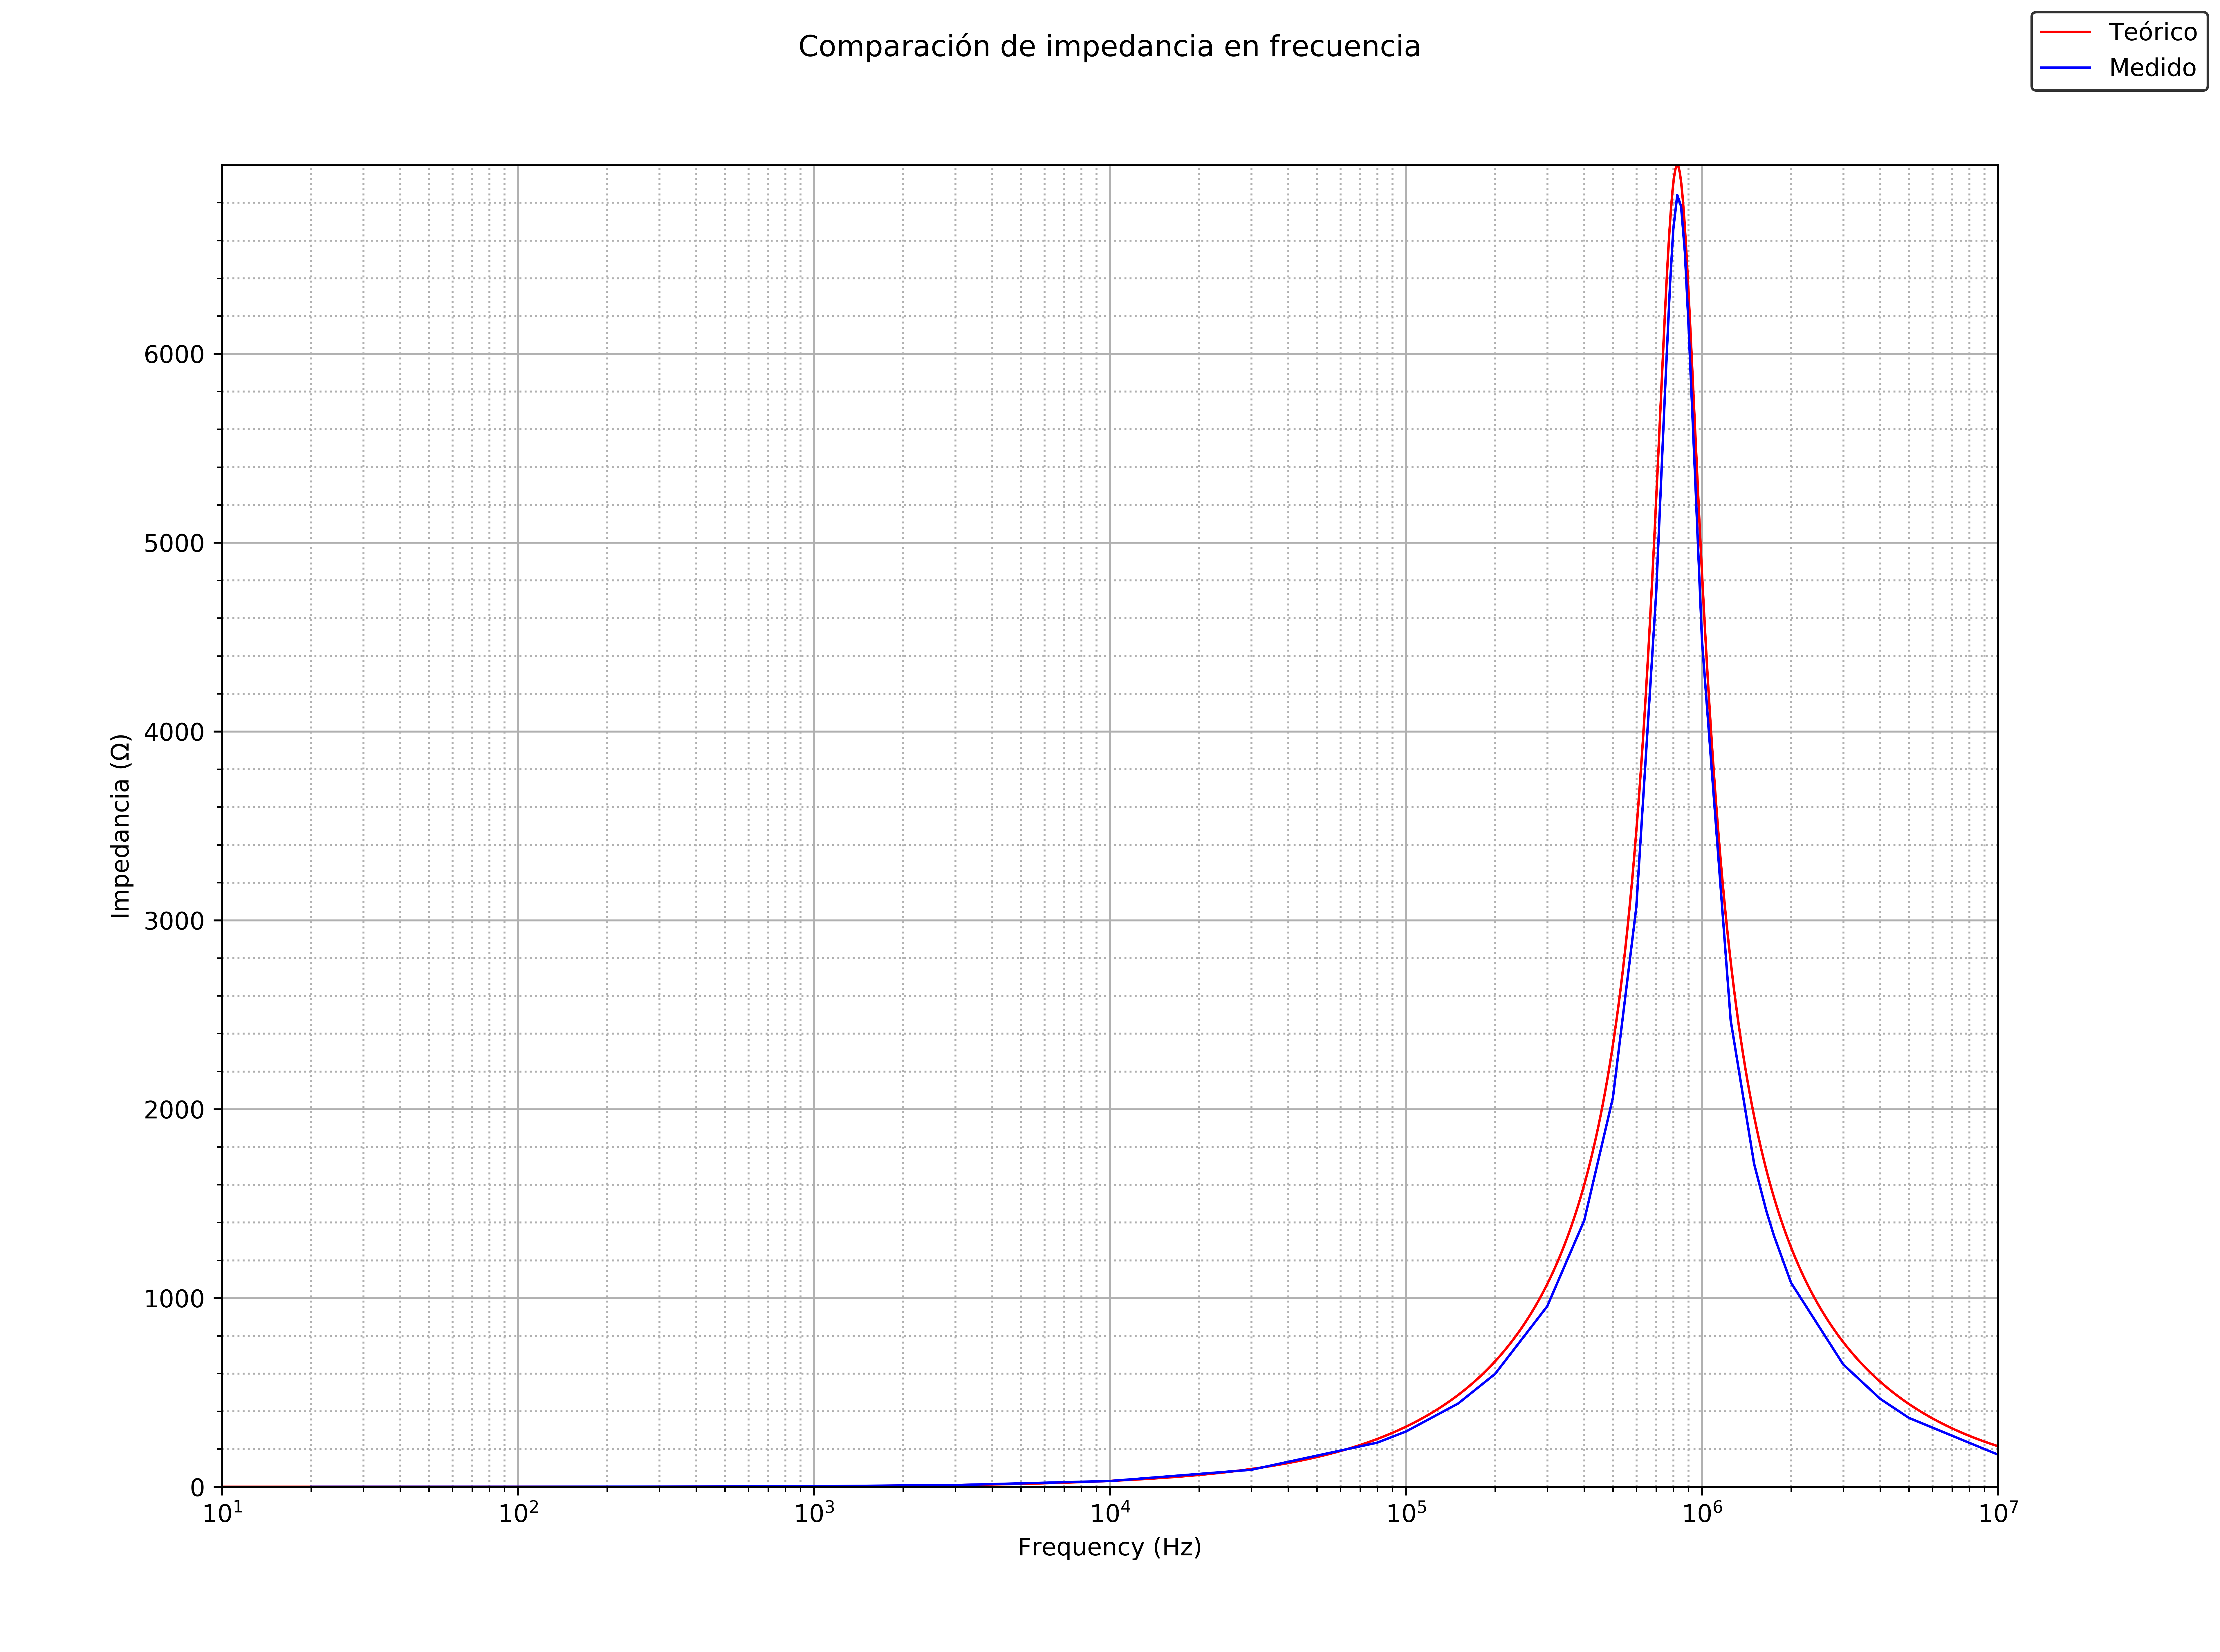
\includegraphics{Recursos/comp_impedancia_ind.png} &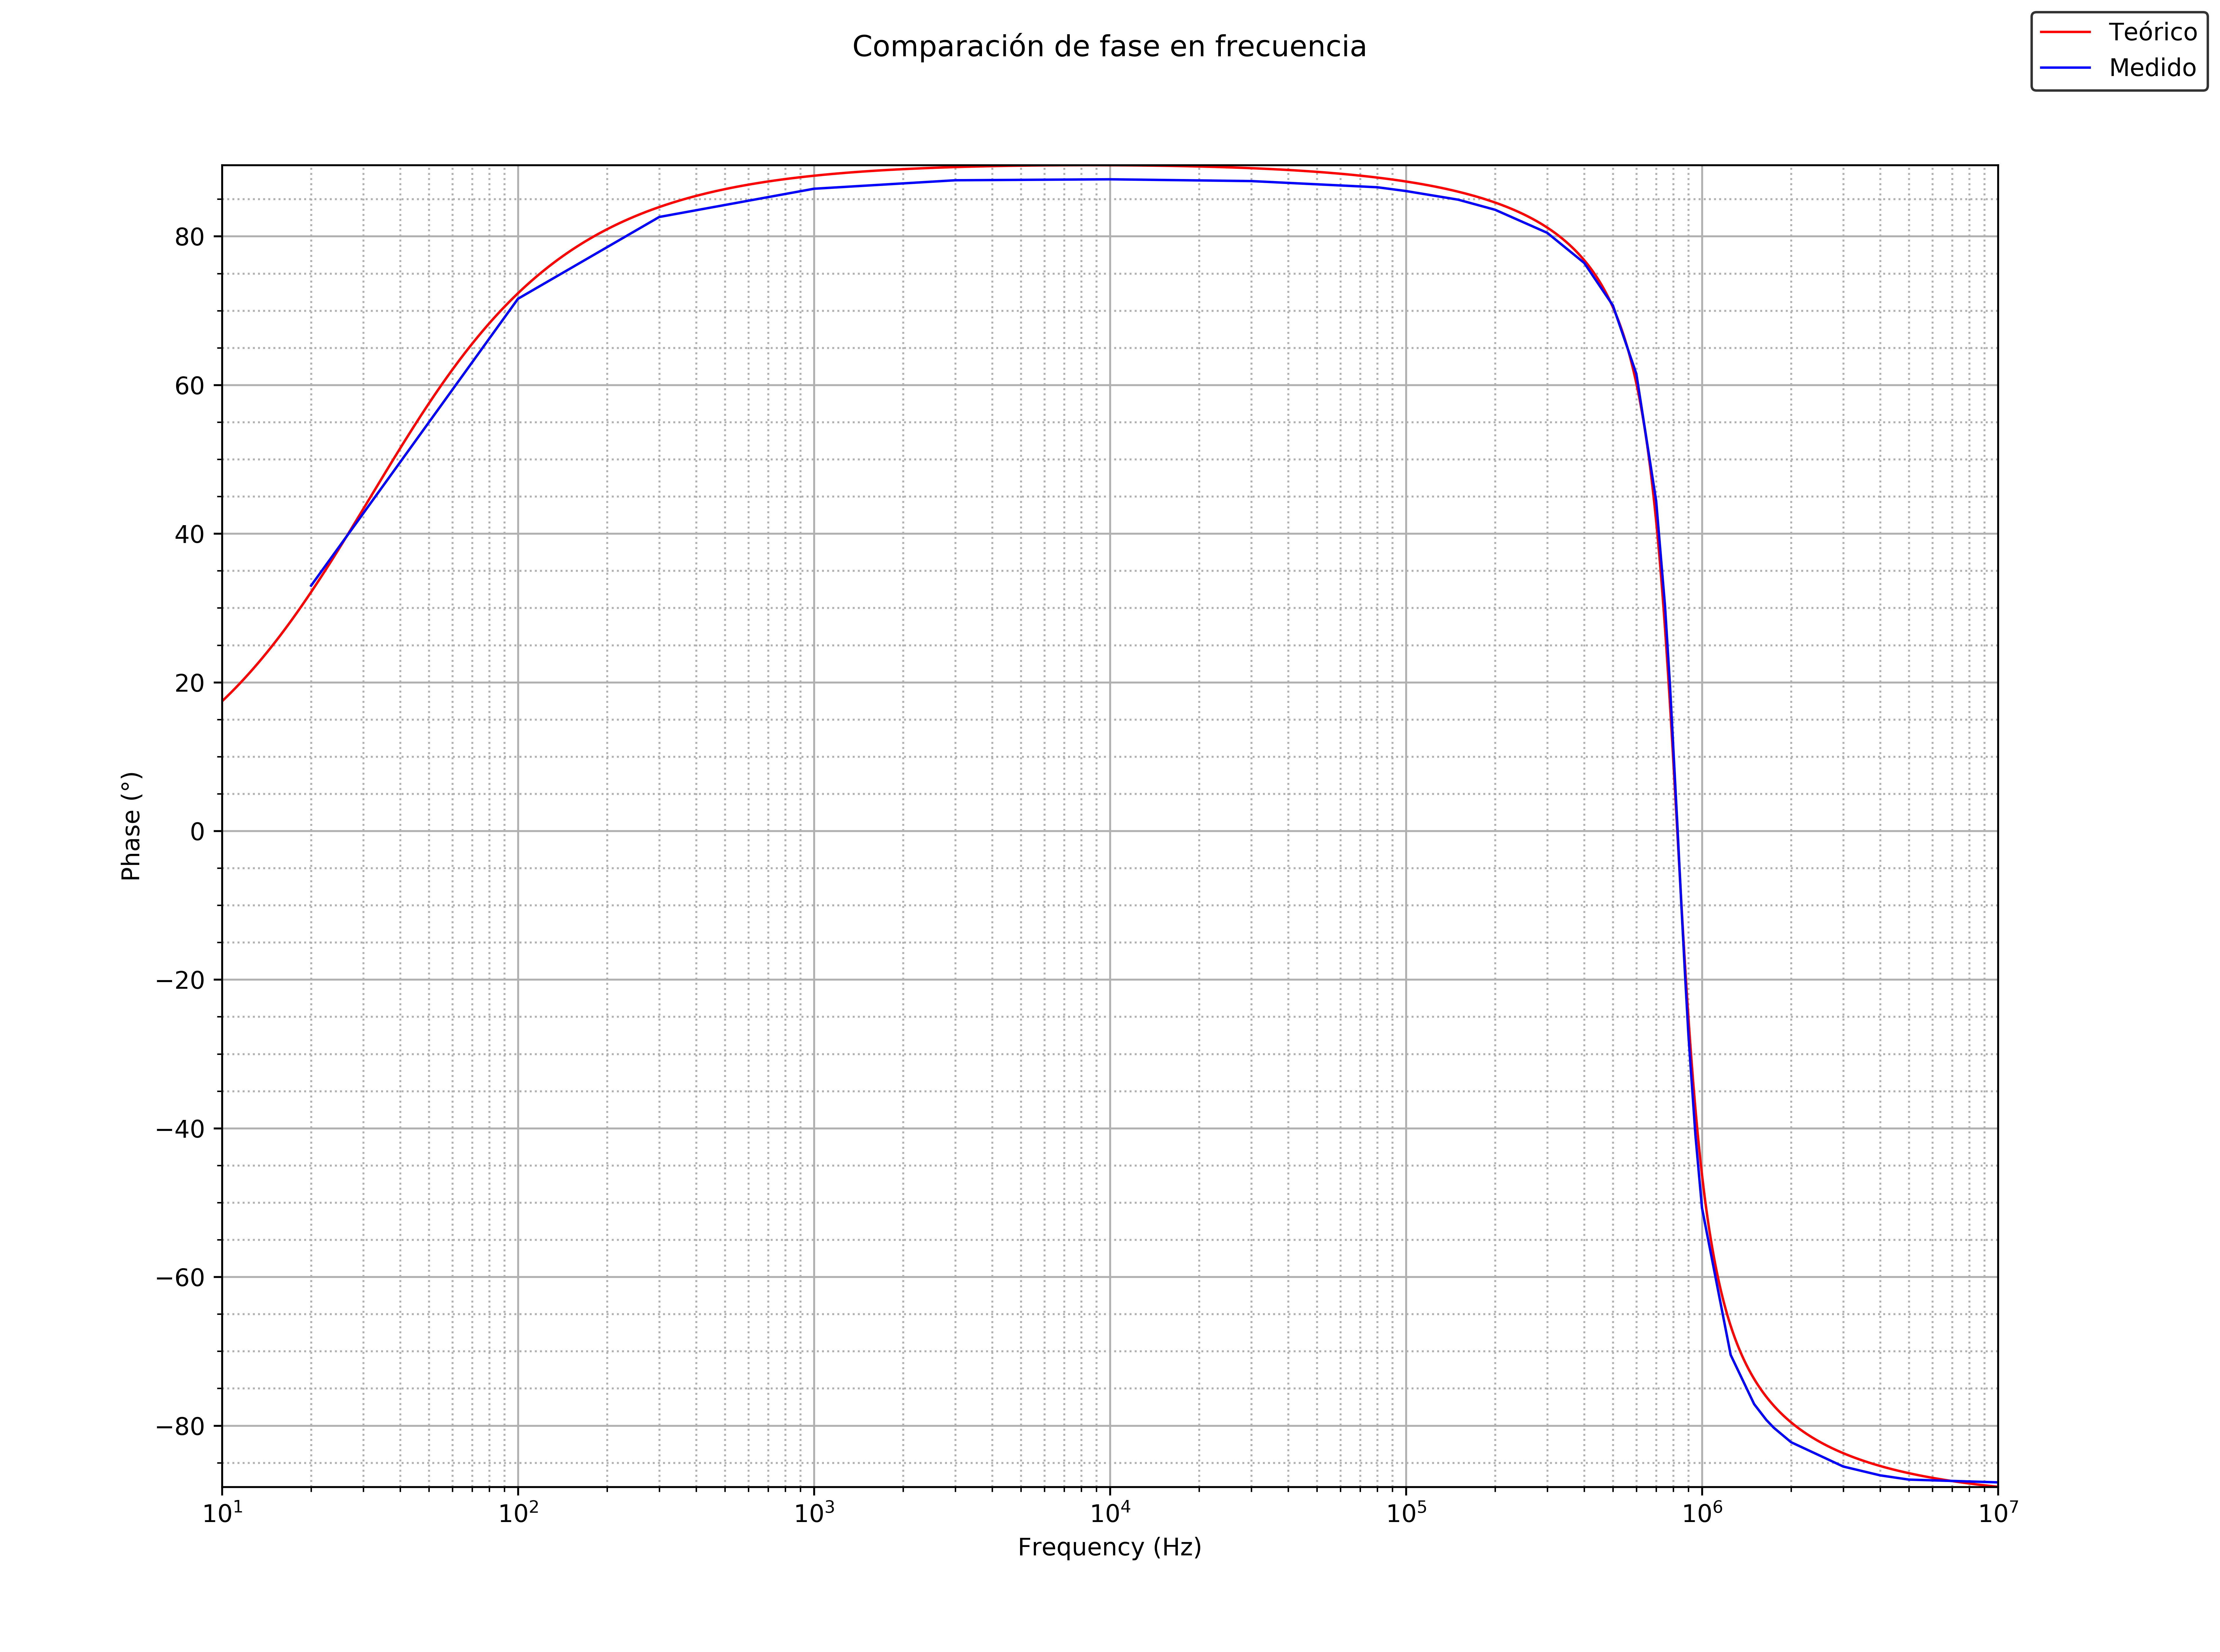
\includegraphics{Recursos/comp_fase_ind.png}
        \end{tabular}
        
    }
    \caption{Comparaci\'on entre mediciones y modelo de impedancia y fase en funci\'on de la frecuencia. }
        \label{fig:Comp_IND}    
\end{figure}

En este caso se observa un ajuste mucho mejor con las curvas medidas.


\subsection{Conclusiones}
Es posible observar en las distintas curvas mostradas en esta secci\'on, las variaciones que los componentes pasivos tienen con la frecuencia. 

Para una frecuencia fuera del rango de operaci\'on, un capacitor puede comportarse como un inductor y viceversa. Es por esto que es de suma importancia, al dise\~nar un circuito de apliaci\'on, elegir correctamente el modelo con el que se trabaja.